\section{Tests und Analysen}
\label{sec:analysen}

In diesem Kapitel wird die Leistungsfähigkeit des gesamten Systems evaluiert. Die Beurteilung erfolgt anhand von realen Videodaten, die dem System während der Trainingsphase nicht präsentiert wurden. Im Fokus steht dabei die Frage, ob die Verbesserungen durch zeitliche Aggregation, den CLAHE-Algorithmus und das asymmetrische Zusammenschneiden zuverlässiger sind als die alleinige Verwendung der Objekterkennung und Klassifikation. Dabei ist es interessant zu sehen, in welchen Szenarien diese Zusätze das System deutlich beeinflussen.

\subsection{Modell-Performance (Training \& Validation)}
Da die YOLO-Modelle einen wesentlichen Teil der Zuverlässigkeit des Systems beeinflussen, werfen wir zuerst einen Blick auf deren isolierte Leistung.

In diesem Unterkapitel wird vor allem auf die Trainingsmetriken eingegangen. Besonders Interessant sind dabei die Verlustfunktionen, welche angeben wie viele Fehler auf den jeweiligen Datensatz (Training oder Validierung) passiert sind. Die Informationen der Wahrheitsmatrizzen geben dabei Einsicht wie viele Objekte erkannt, fälschlicherweise erkannt oder vom Modell erfunden wurden.

\subsubsection{Leistung der Objekterkennung (Katzengesicht)}
Die Trainingsmetriken (Abbildung \ref{fig:training_det}) für den Katzengesicht-Detektor, zeigen einen kontinuierlich sinkenden Trainingsfehler (\emph{engl. Loss}) und eine hohe Genauigkeit (\emph{engl. Precision}) in der Validierung im Verlauf von 100 Epochen.

\begin{figure}[H]
    \centering
    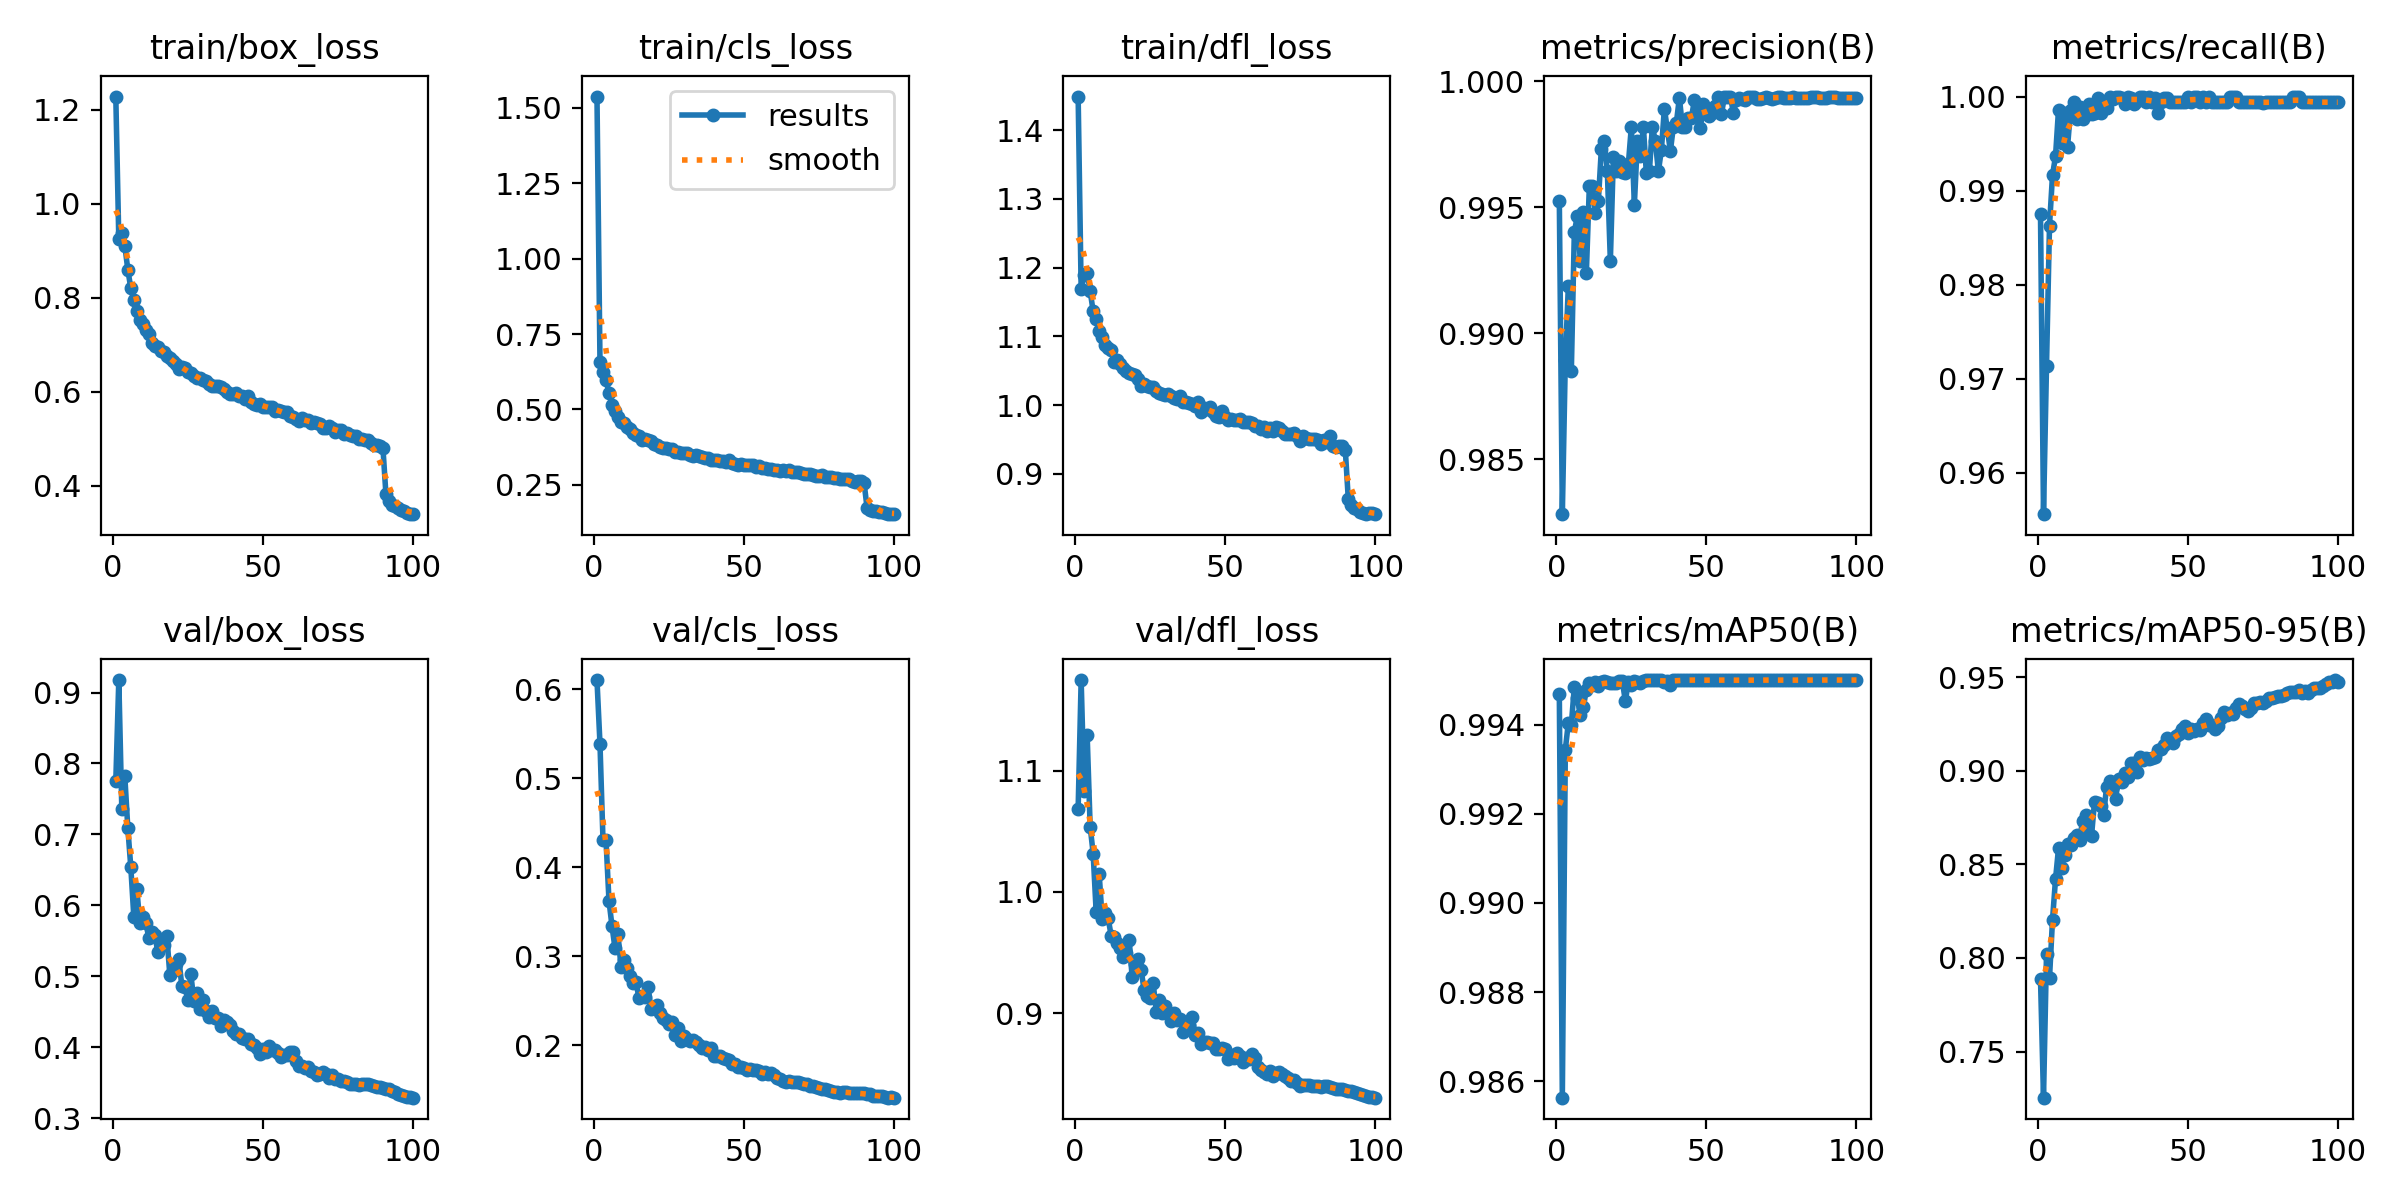
\includegraphics[width=0.8\textwidth]{images/results.png}
    \caption{Trainingsverlauf und Metriken des YOLO-Objektdetektors.}
    \label{fig:training_det}
\end{figure}

Die Wahrheitsmatrix (\emph{engl. Confusion Matrix}) der Objekterkennung (Abbildung \ref{fig:confusion_det}) verdeutlicht die Präzision bei der Lokalisierung. Sie zeigt, dass bei der Validierung 1.676 Katzengesichter korrekt erkannt wurden. Das Modell hat jedoch zwei Katzengesichter erkannt, obwohl dort keines war, und eines hat es komplett übersehen. Die Matrix belegt also dass der Detektor nahezu fehlerfrei auf den Validierungsdaten funktionierte.

\begin{figure}[H]
    \centering
    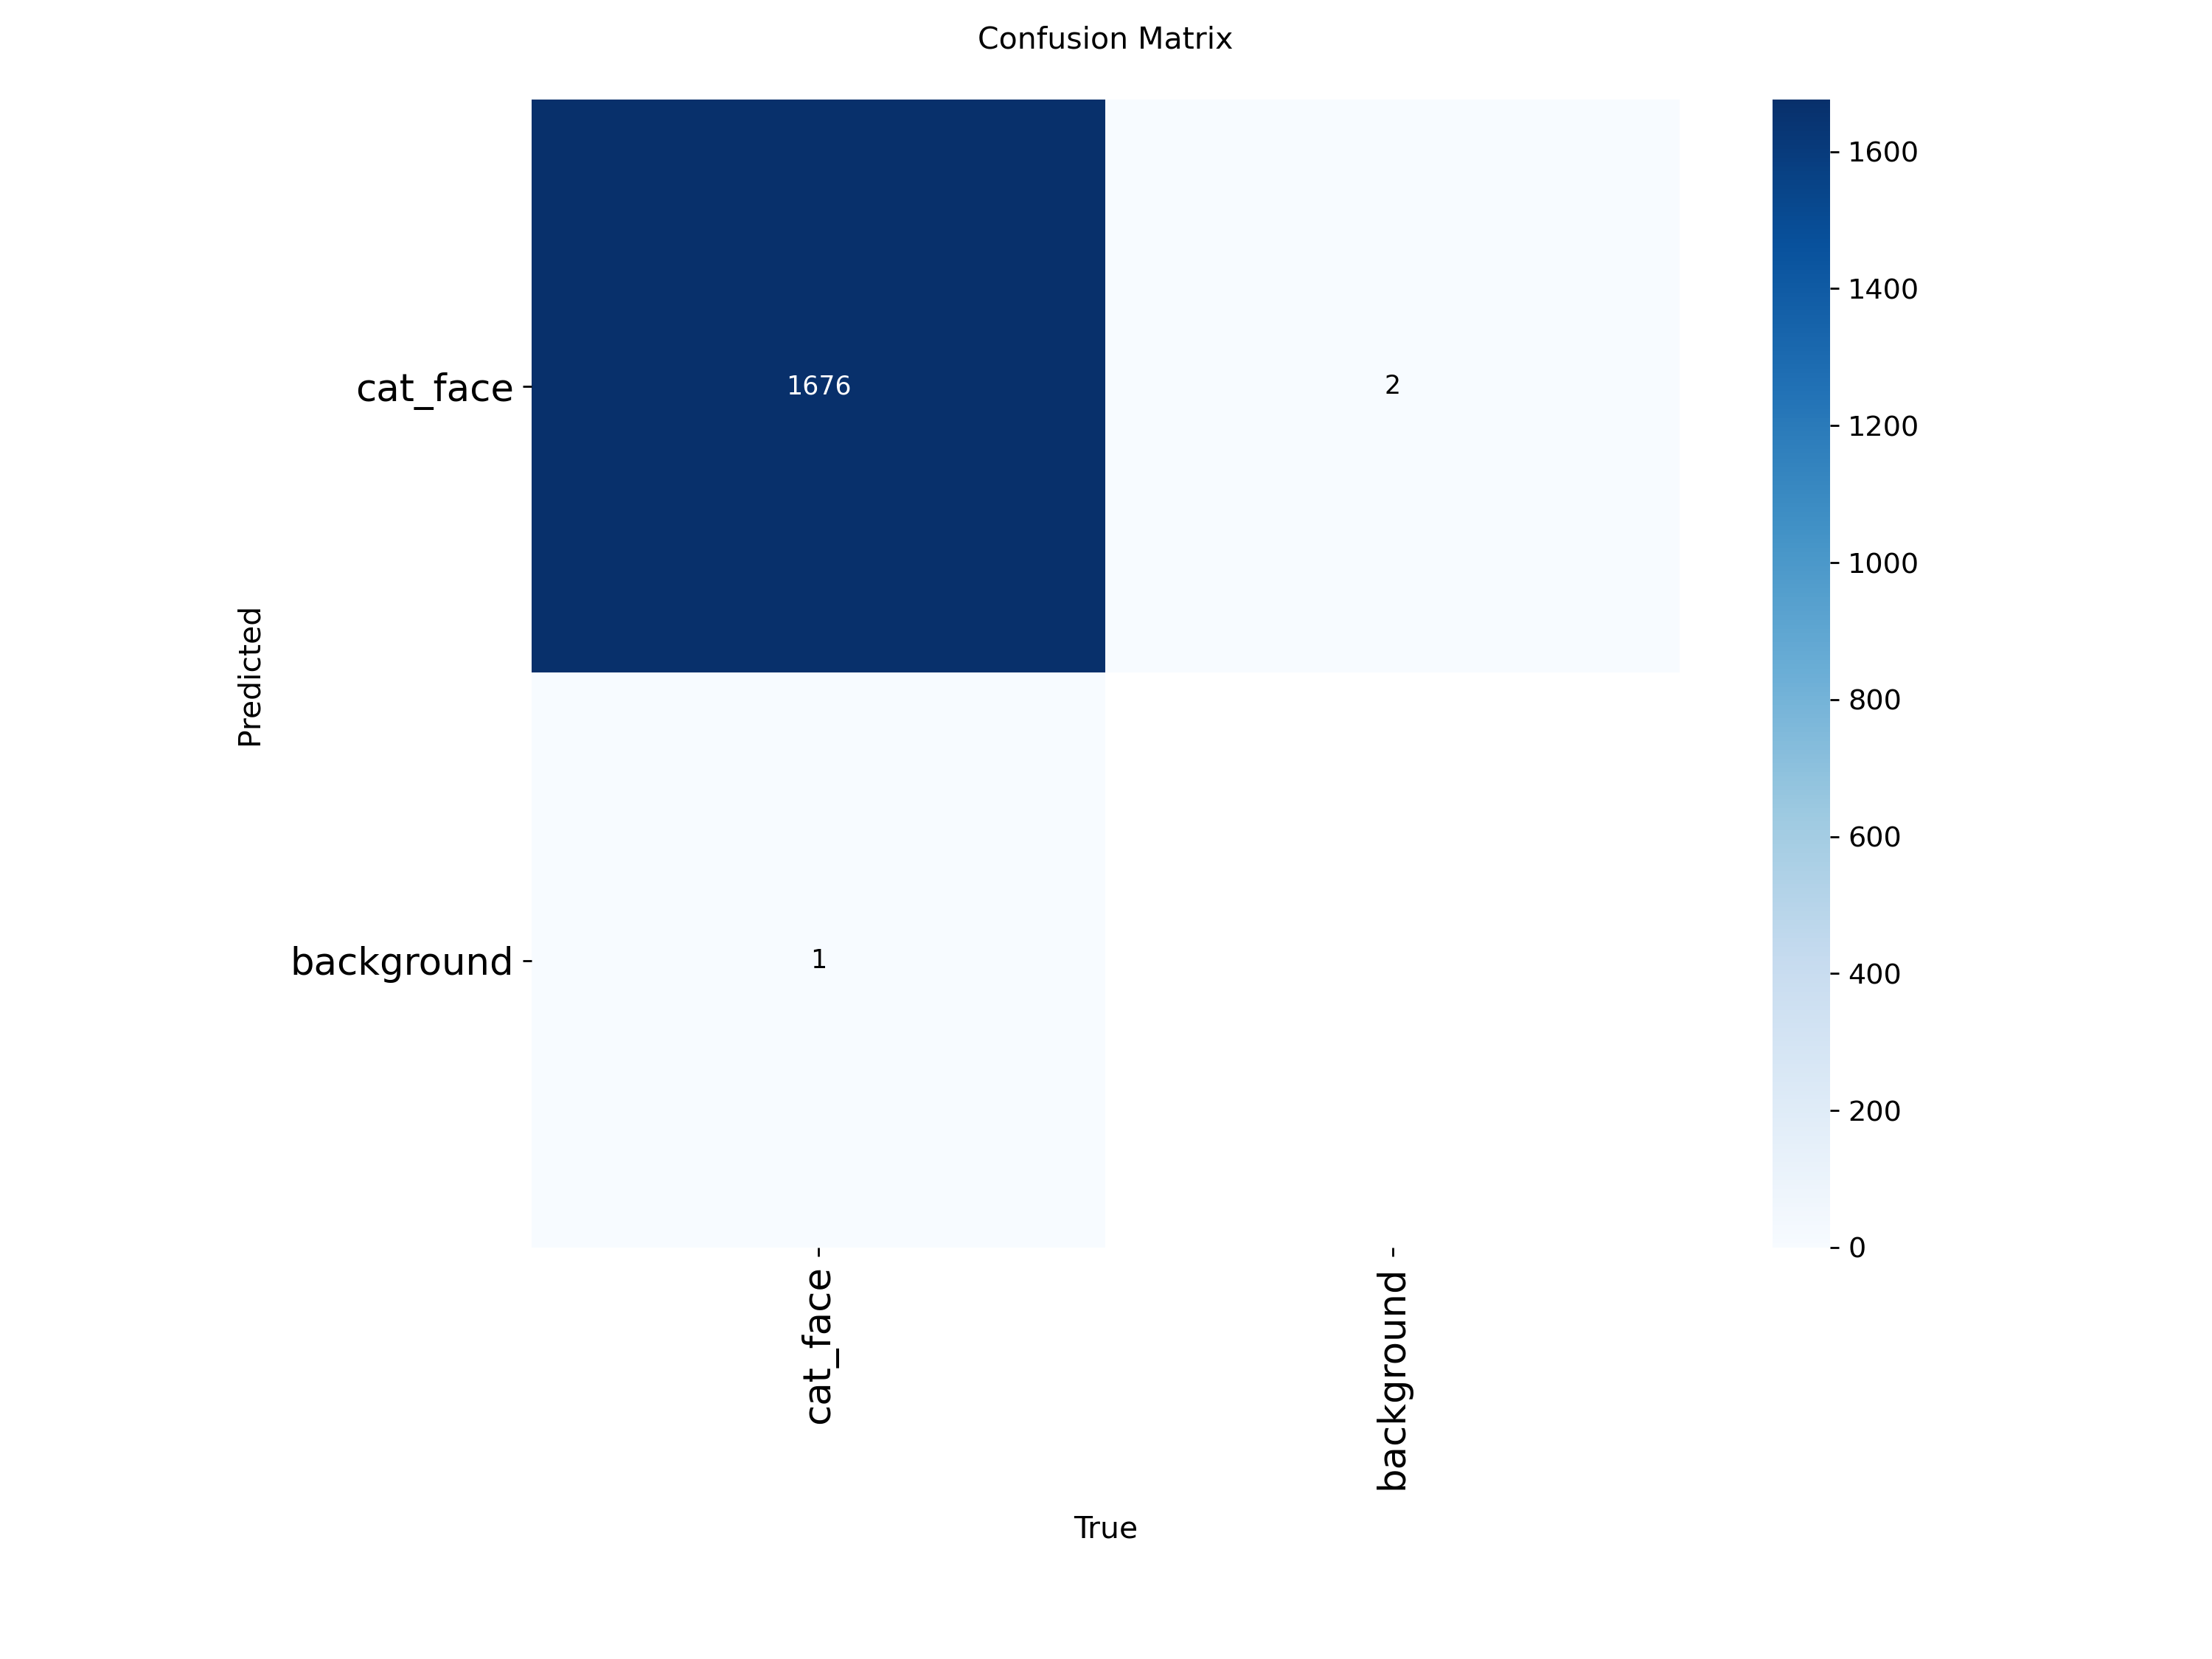
\includegraphics[width=0.6\textwidth]{images/confusion_matrix.png}
    \caption{Wahrheitsmatrix (Detektor).}
    \label{fig:confusion_det}
\end{figure}

Eine wichtige Metrik, welche auch auf den Validierungsdaten beruht, ist die Präzision-Trefferquote-Kurve (\emph{engl. Precision-Recall-Curve}), sie gibt das Verhältnis zwischen richtig erkannten Objekten und Fehlalarmen an wie sicher  das Modell ist. In diesem Fall zeigt der Verlauf, dass das Modell extrem sicher ist und nicht raten muss, wenn es ein Katzengesicht sieht.

\begin{figure}[H]
    \centering
    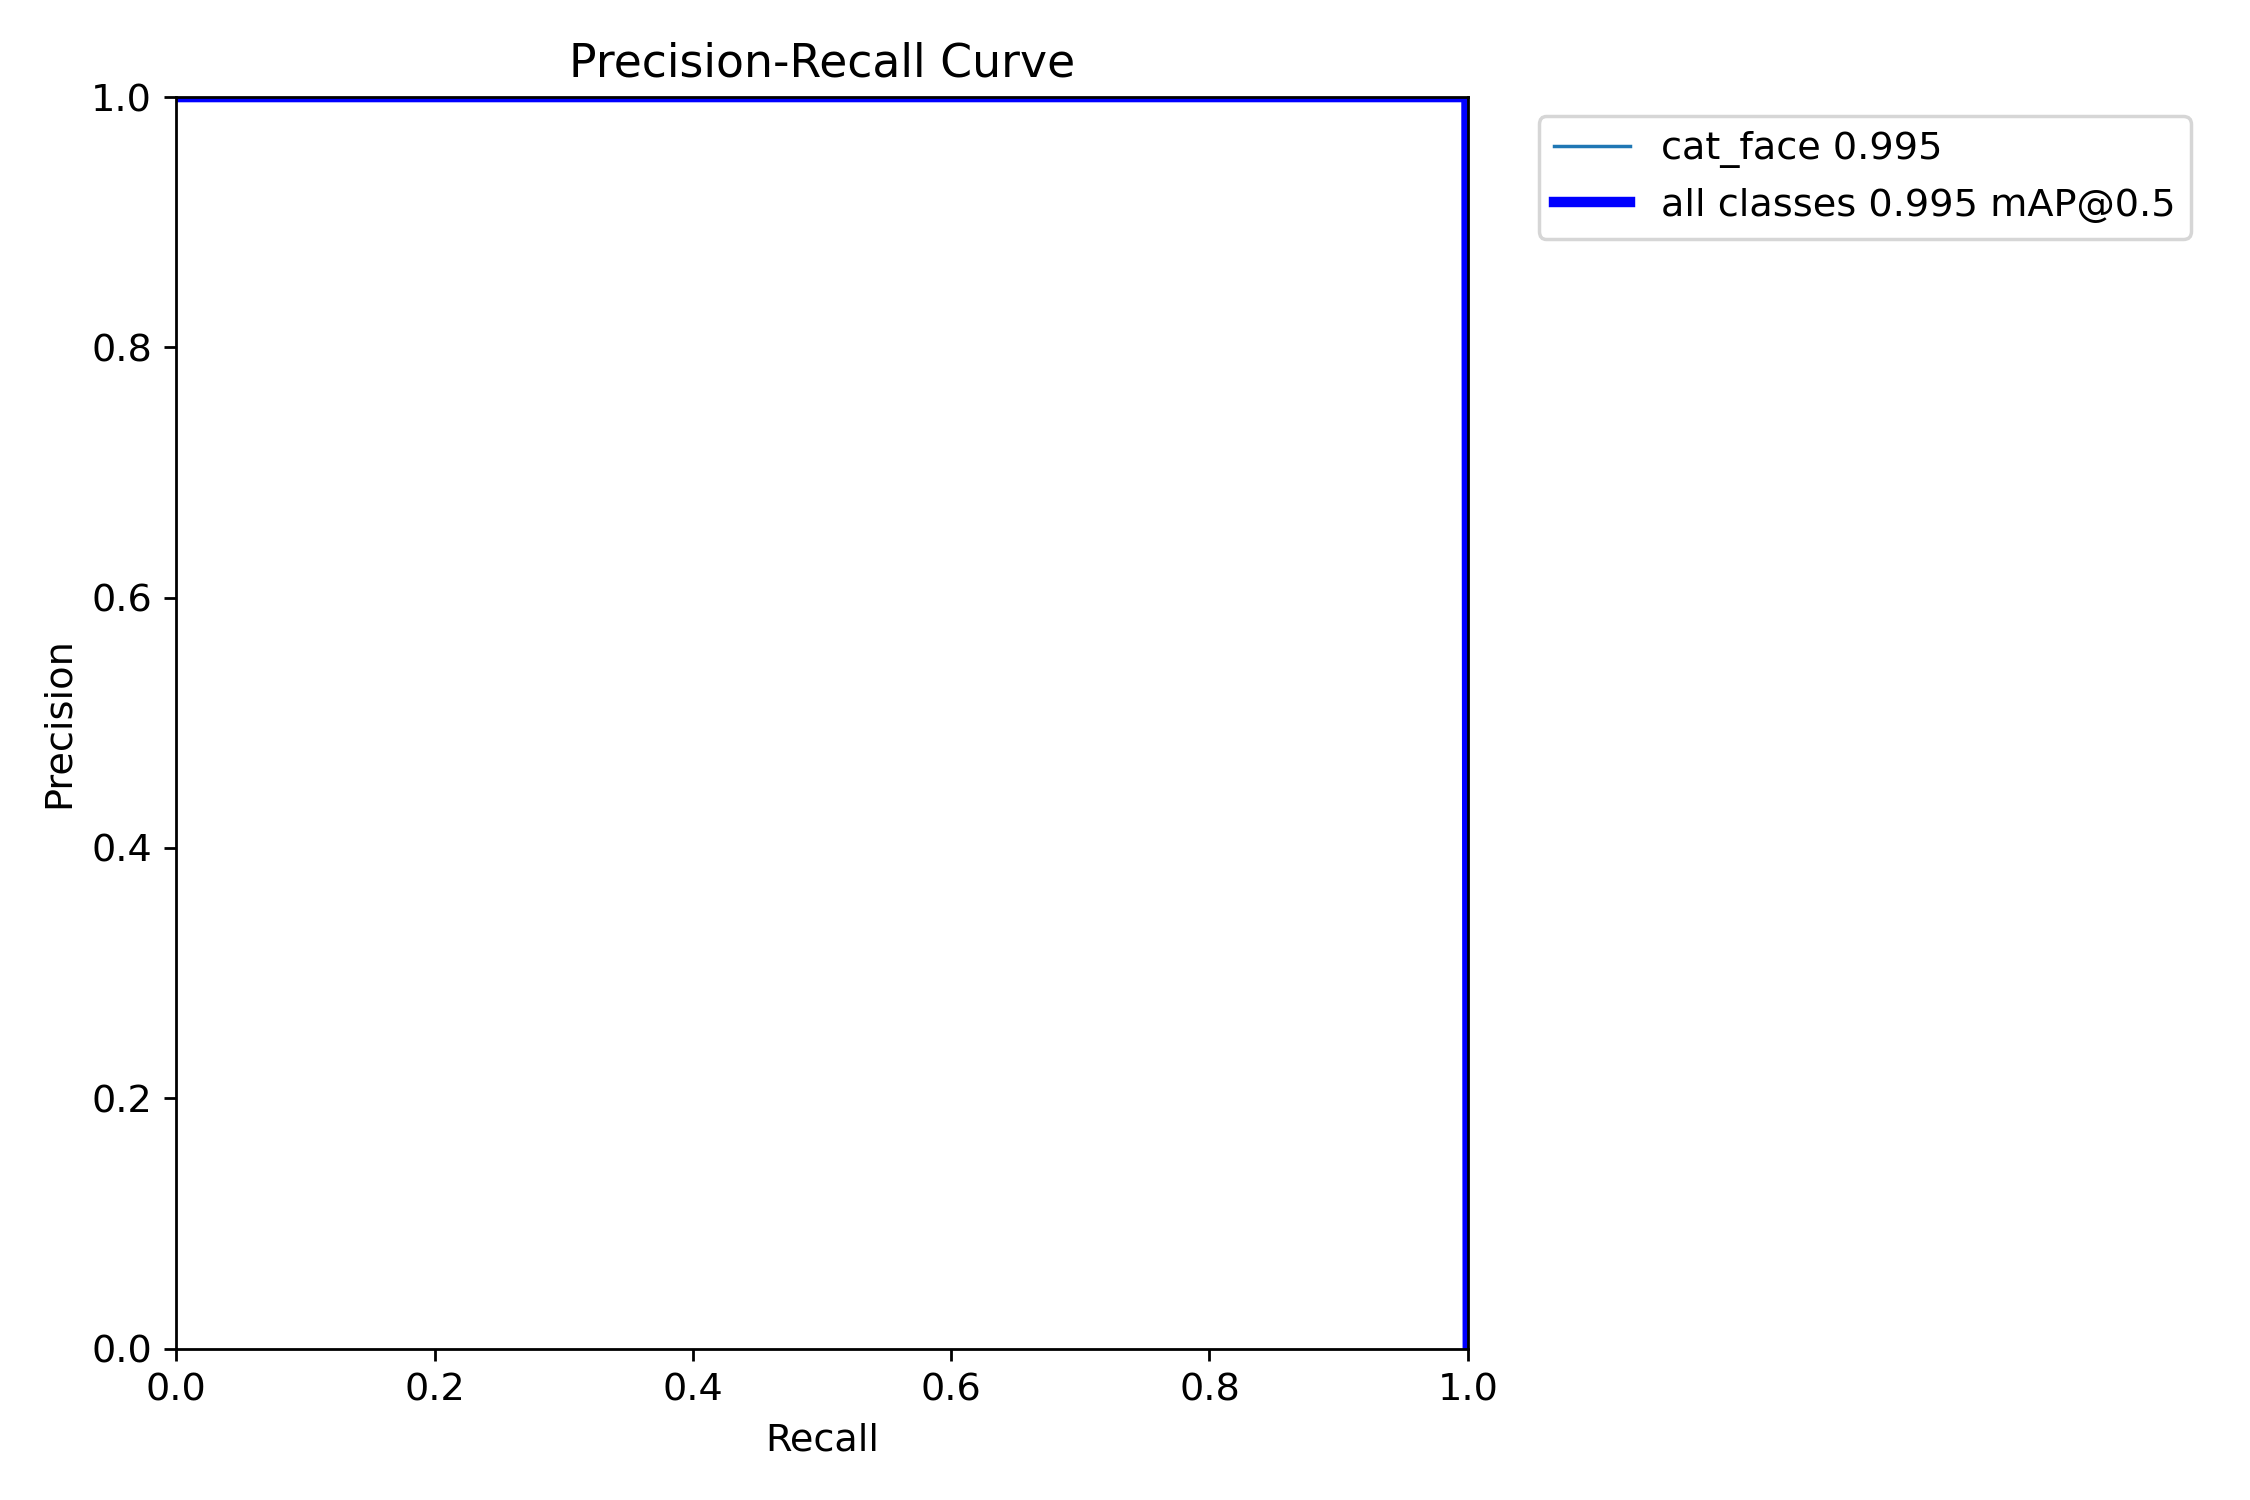
\includegraphics[width=0.6\textwidth]{images/BoxPR_curve.png}
    \caption{Präzision-Trefferquote-Kurve (\emph{engl. Precision-Recall-Curve}).}
    \label{fig:pr_curve_det}
\end{figure}

Die F1-Maß-Kurve (Abbildung \ref{fig:f1_curve_det}) zeigt wie sich die Leistung des Modells bei Änderung des Konfidenzschwellenwerts \cite{ultralytics_confidence} verändert. Dadurch können wir den optimalen Schwellenwert für den realen Betrieb des Modells ermitteln. Da die Kurve bis $\approx 0,85$ flach bleibt, d.h. hier wird keine Katze übersehen, fällt sie $> 0{,}85$ stark ab. Das zeigt, dass ab diesem Schwellenwert auch reale Katzen leicht übersehen werden. In der Praxis zeigt sich, dass bei einem Konfidenzschwellwert von $\approx 0,75$ ein gutes Verhältnis zwischen „Katze wird nicht erkannt” und „es wird eine Katze erkannt, wo sich keine befindet” entsteht.

\begin{figure}[H]
    \centering
    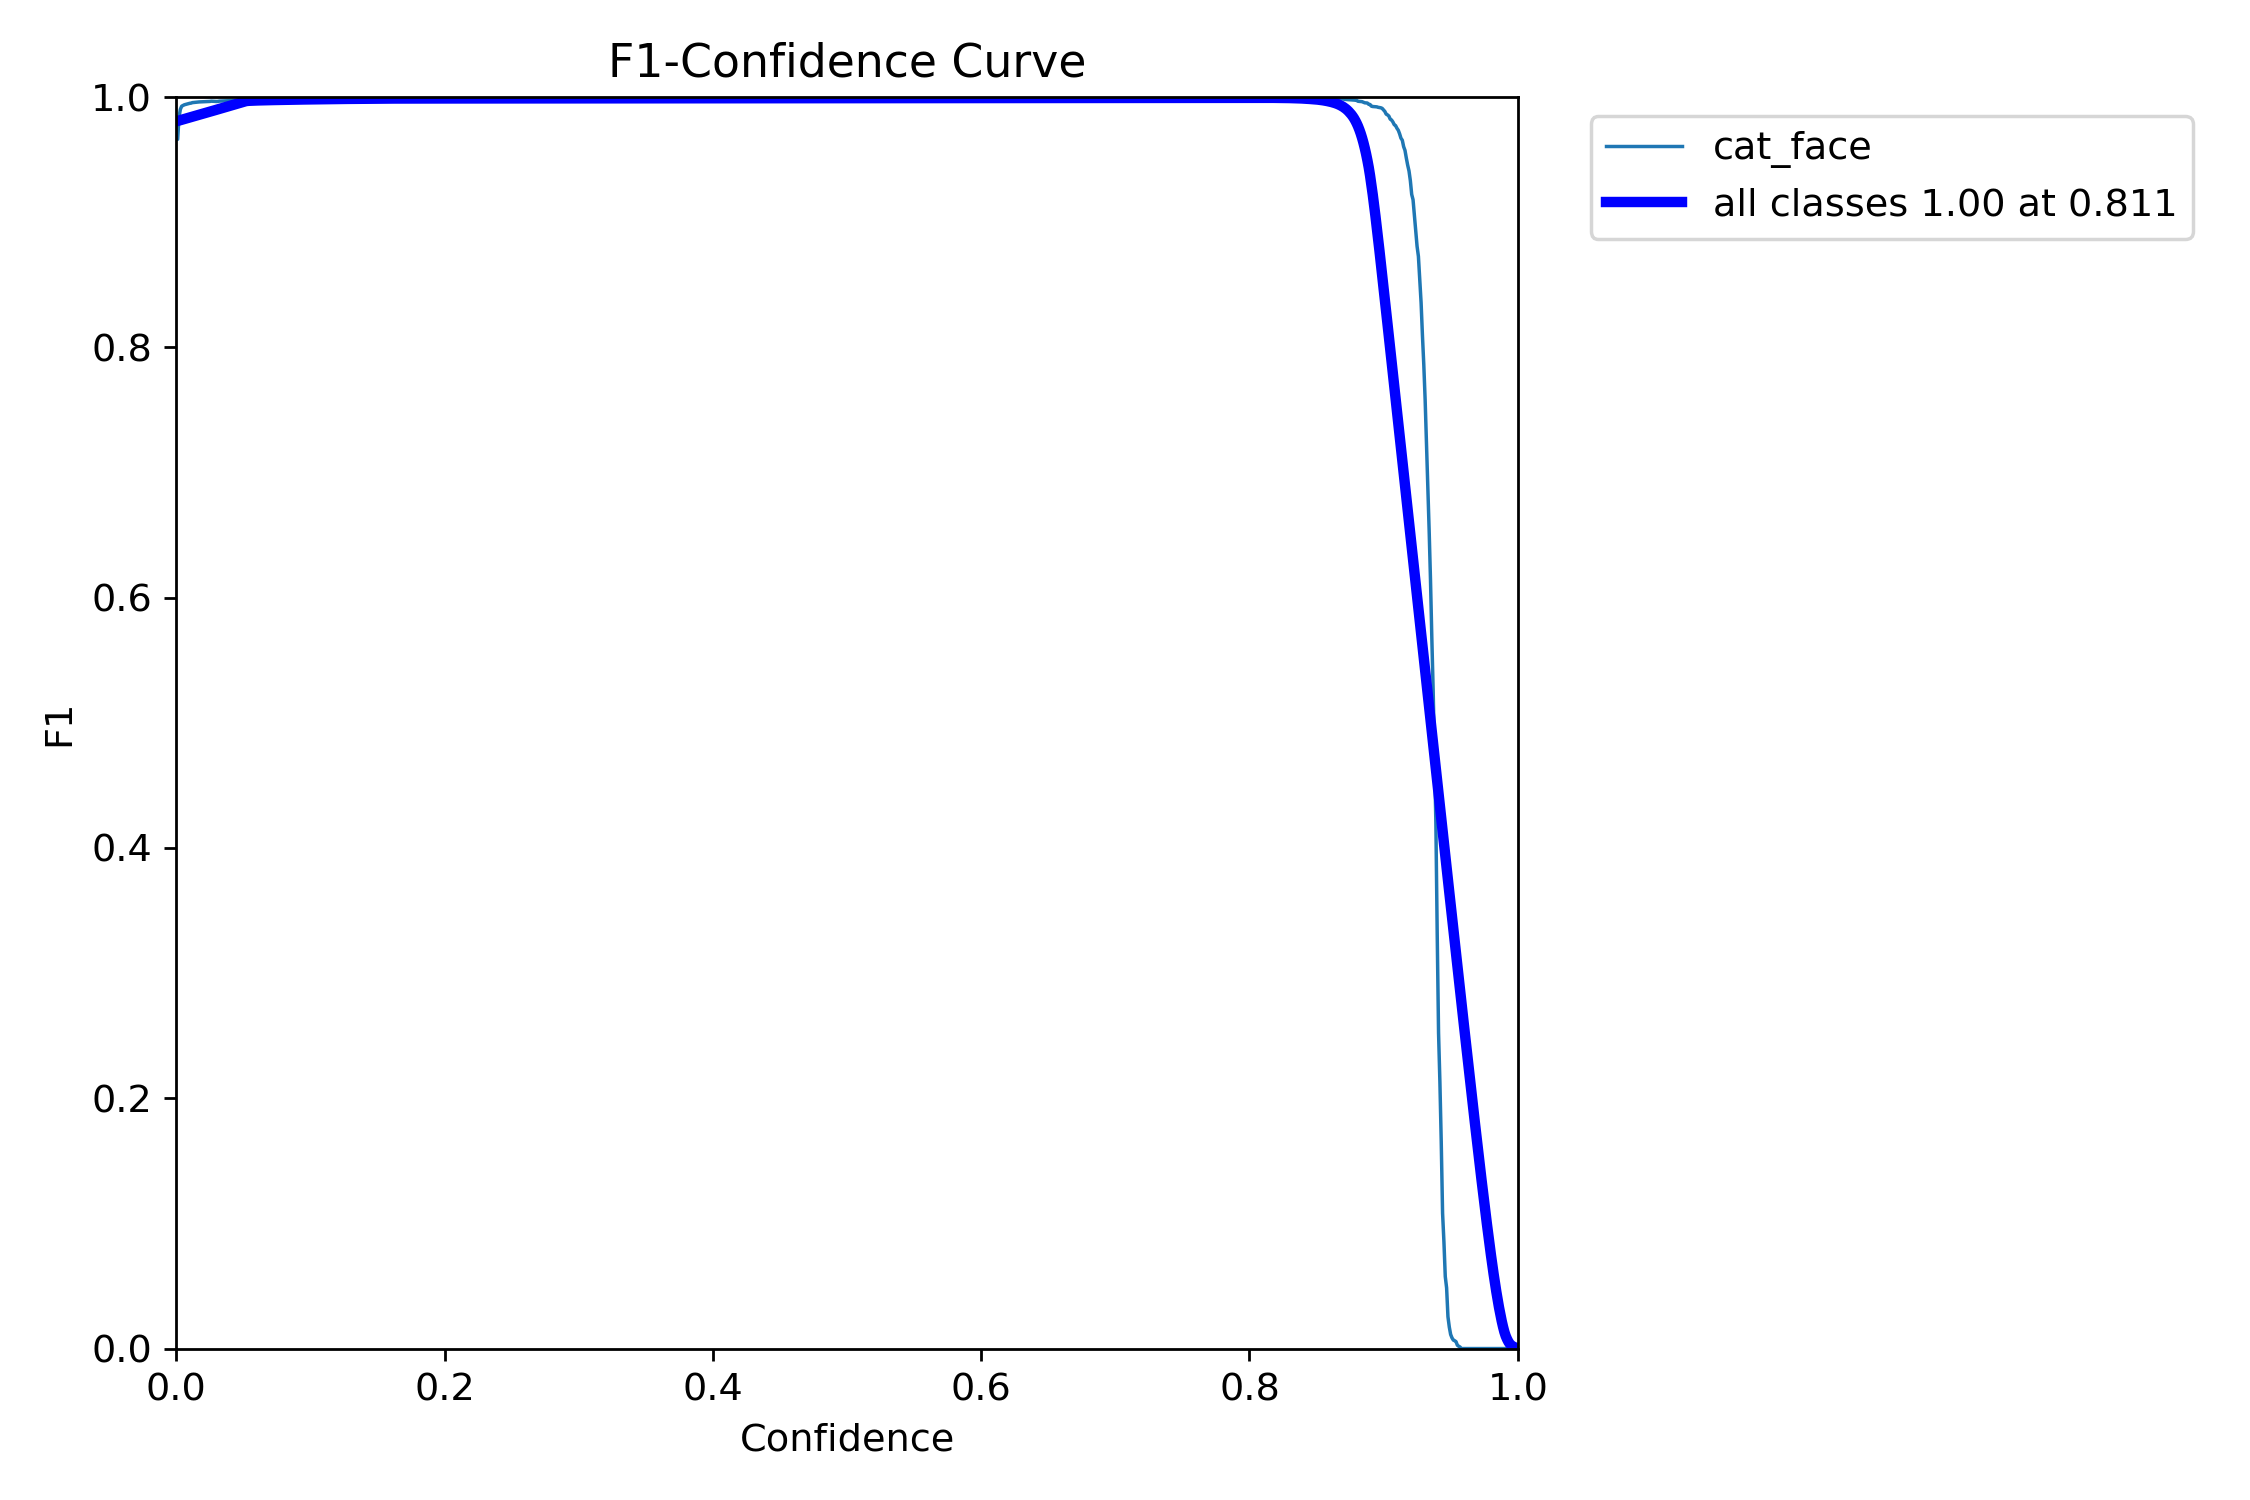
\includegraphics[width=0.6\textwidth]{images/BoxF1_curve.png}
    \caption{F1-Maß-Kurve.}
    \label{fig:f1_curve_det}
\end{figure}

Die Abbildung \ref{fig:val_pred_det} liefert einen Eindruck auf die Erkennungsleistung des Modells, wenn man es auf die Validierungsdaten ansetzt.

\begin{figure}[H]
    \centering
    \includegraphics[width=0.8\textwidth]{images/val_batch0_pred.jpg}
    \caption{Vorhersagen des Detektors auf dem Validierungsdatensatz.}
    \label{fig:val_pred_det}
\end{figure}

\subsubsection{Leistung der Bildklassifikation (Beute)}
Die folgenden Trainingsmetriken des Klassifikators zeigen, dass das Modell seine Aufgabe erfolgreich gelernt hat.
Beim betrachten der Verlustfunktionen wird ersichtlich, dass das Modell über die Epochen weniger Fehler sowohl bei Training als auch Validierung macht, daraus können wir schließen, dass der Klassifikator lernt ohne sich dabei zu viel auf den Trainingsdatensatz anpasst.

\begin{figure}[H]
    \centering
    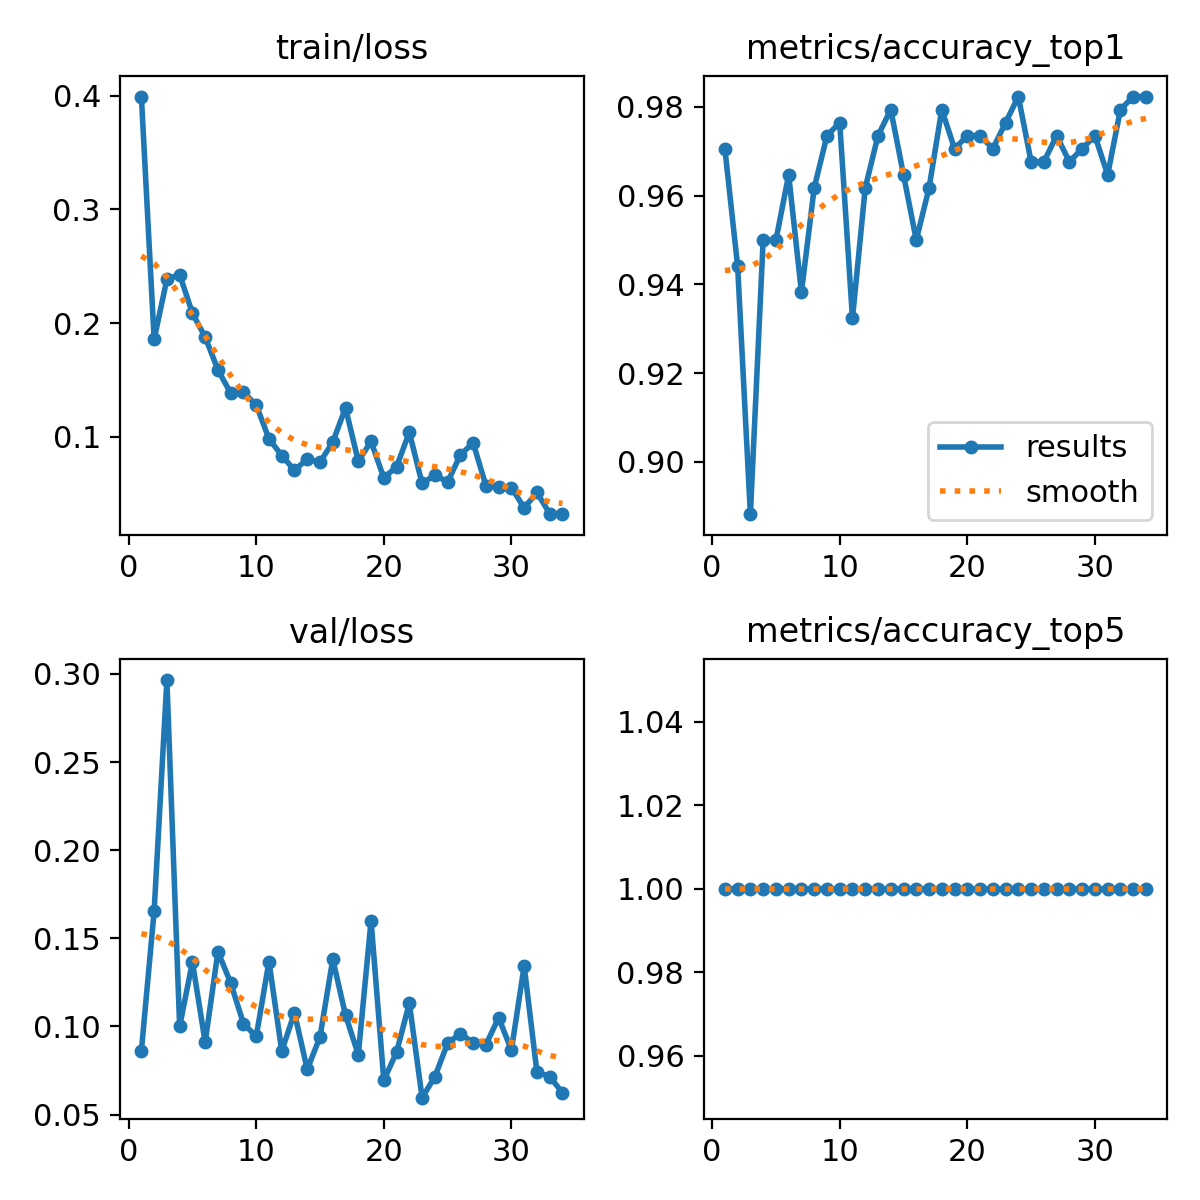
\includegraphics[width=0.8\textwidth]{images/results_cls.png}
    \caption{Trainingsverlauf und Metriken des YOLO-Klassifikators.}
    \label{fig:training_cls}
\end{figure}

Wenn man einen Blick auf die Wahrheitsmatrix (Abbildung \ref{fig:confusion_cls}) wirft, zeigt sich, dass das Modell auf den Validierungsdatensatz großartig funktionierte. Bei den insgesamt 335 Fotos, gab es nur 5 Fehler bei der binären Entscheidung \glqq Beute\grqq\ und \glqq Keine Beute\grqq.

\begin{figure}[H]
    \centering
    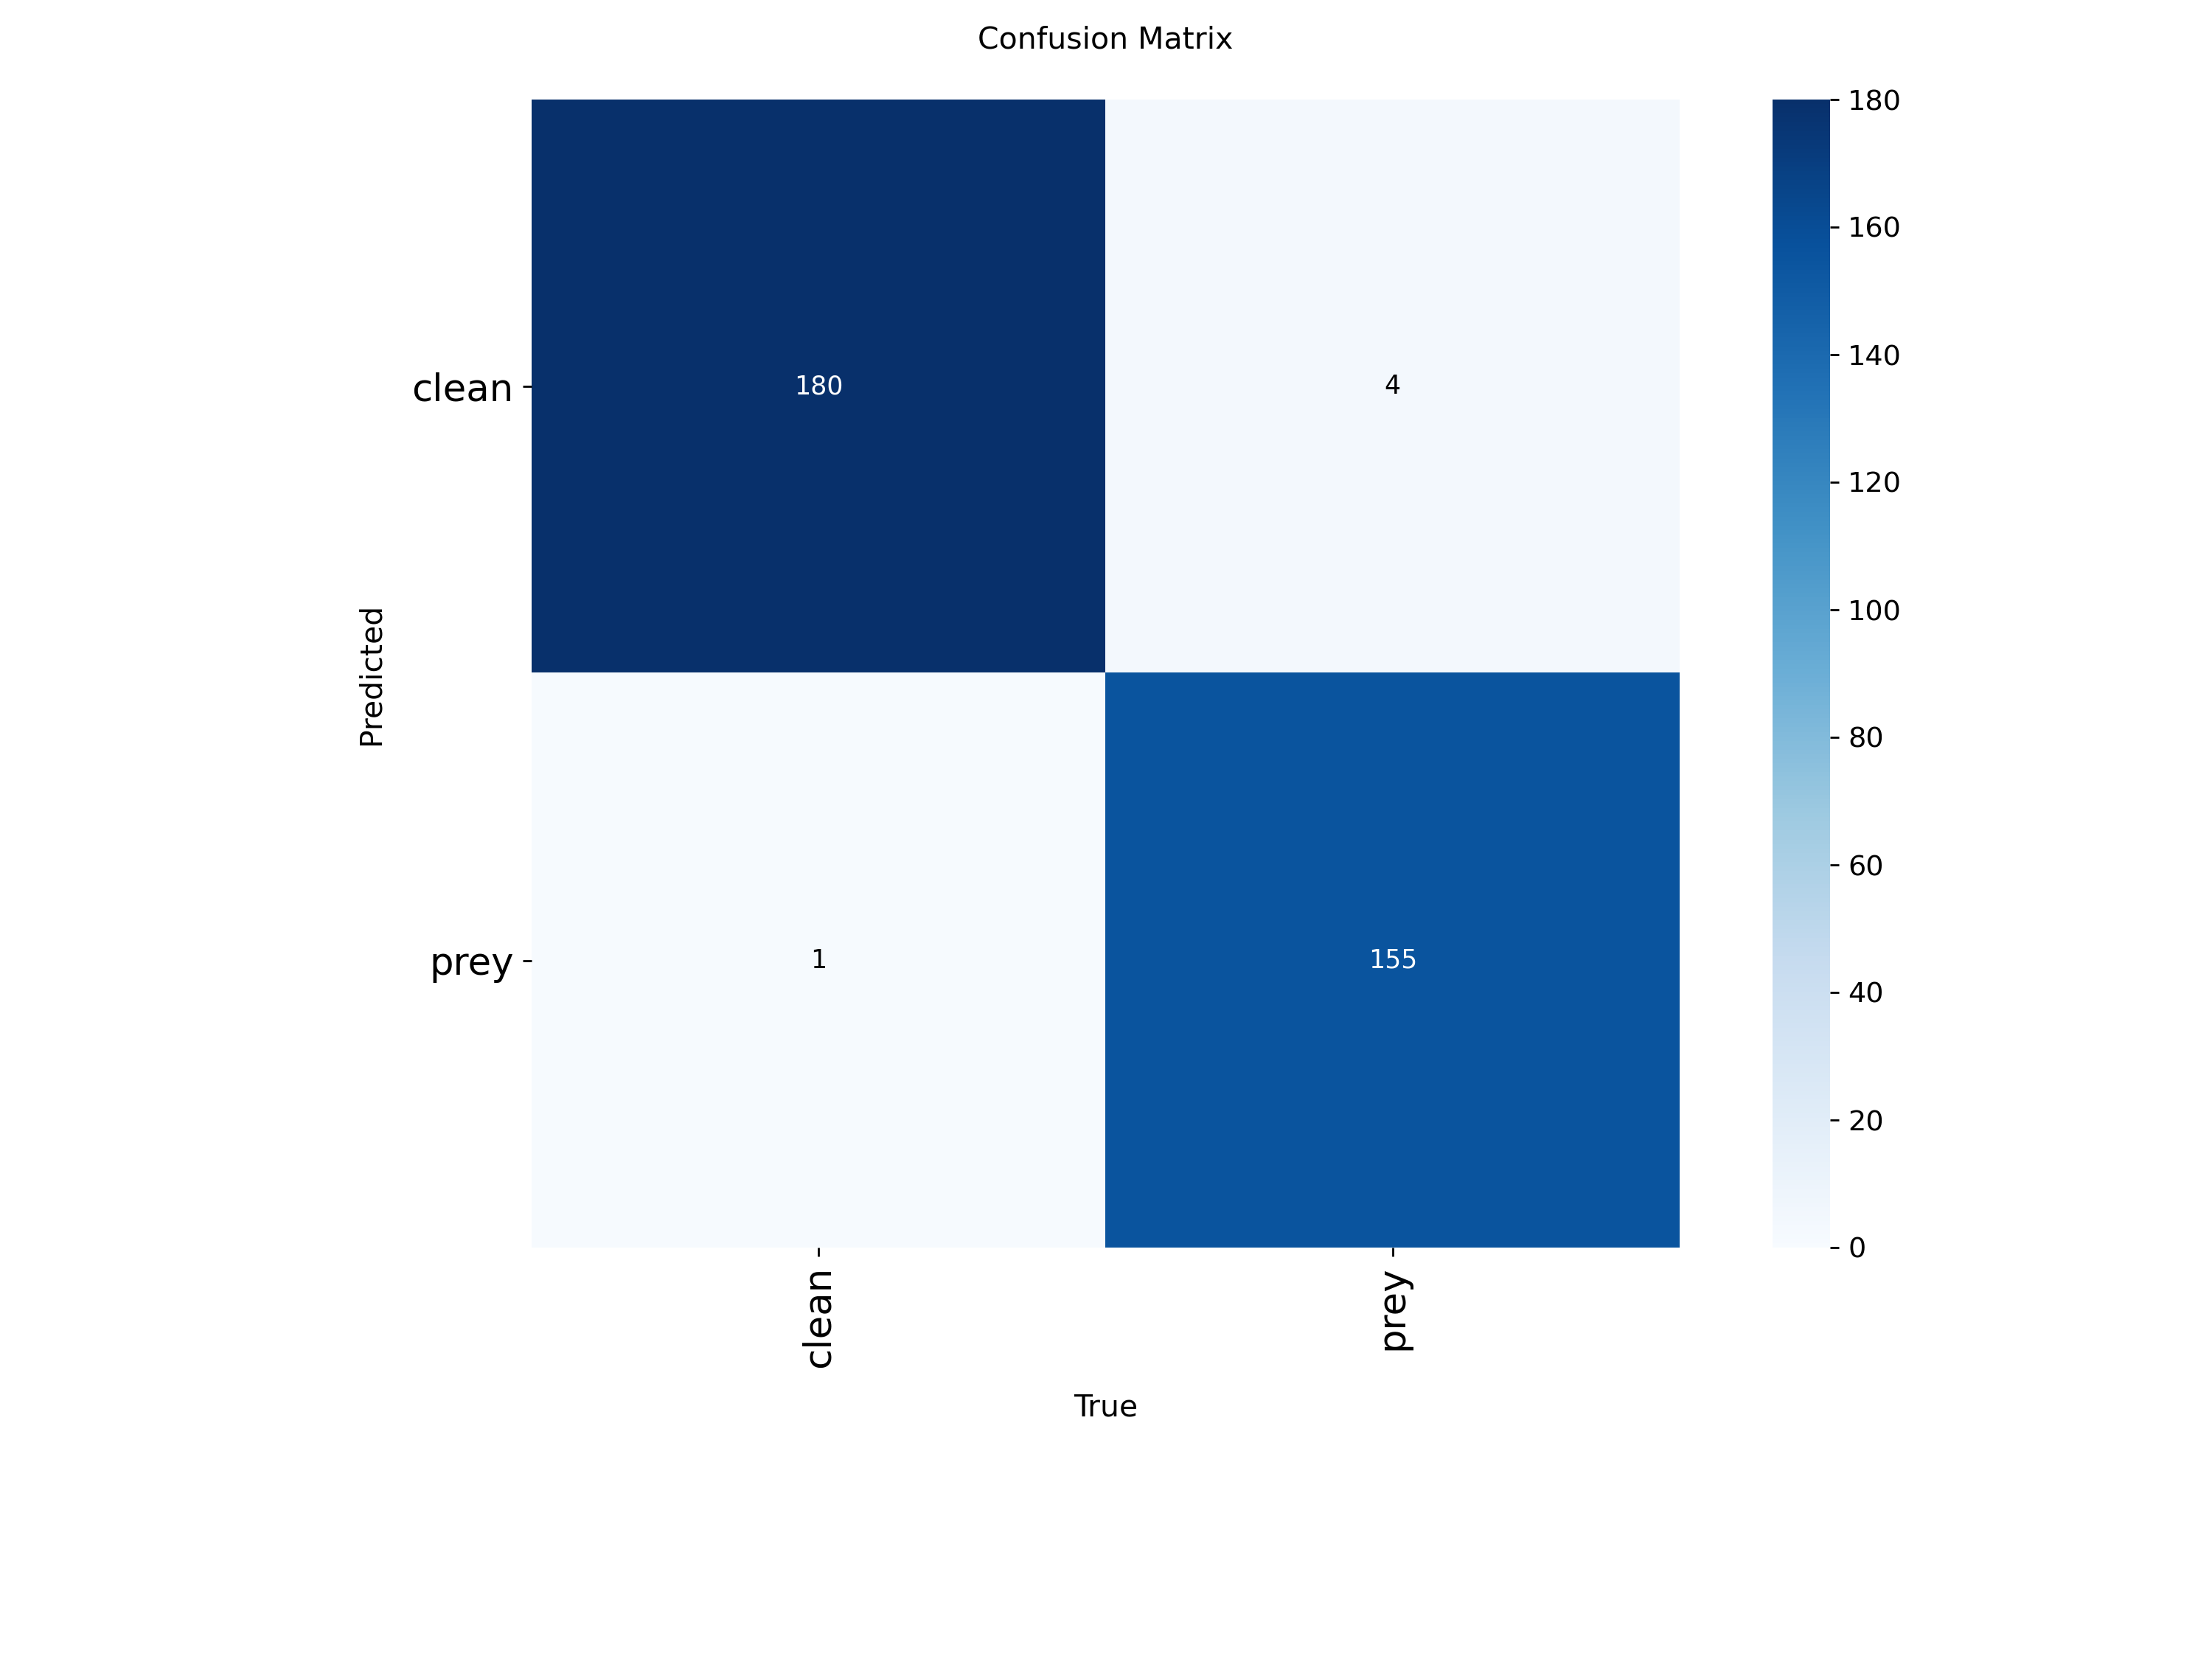
\includegraphics[width=0.6\textwidth]{images/confusion_matrix_cls.png}
    \caption{Confusion Matrix des Klassifikators auf dem Validierungsdatensatz.}
    \label{fig:confusion_cls}
\end{figure}

Mithilfe der Abbildung \ref{fig:val_pred_cls} kann man gut erkennen wie gut das Modell auf unbekannten Daten funktioniert.

\begin{figure}[H]
    \centering
    \includegraphics[width=0.8\textwidth]{images/val_batch0_pred_cls.jpg}
    \caption{Beispielhafte Vorhersagen des Klassifikators auf dem Validierungsdatensatz.}
    \label{fig:val_pred_cls}
\end{figure}

Rein auf dem Papier würden diese Modelle fast fehlerfreie Aussagen treffen. Die entscheidende Frage ist jedoch, wie verhält sich das System im Praxiseinsatz und welche Vorteile bietet die Verarbeitungskette gegenüber der reinen Detektion und Klassifikation.

\subsection{Evaluationsmethodik und Datensatz}

Die Testbasis für das System bilden insgesamt 7 Videosequenzen, die sich auf zwei Kategorien aufteilen. Die Dateinamen der Kategorien geben Aufschluss wie viele Katzen und in welcher Farbe in dem Video vorkommen.

\begin{itemize}
    \item \textbf{Positive Samples (Mit Beute):} 4 Videos (\texttt{black.mp4}, \texttt{orange.mp4}, \texttt{orange2.mp4}, \texttt{two\_cats\_black\_white.mp4})
    \item \textbf{Negative Samples (Ohne Beute):} 3 Videos (\texttt{black.mp4}, \texttt{orange.mp4}, \texttt{two\_cats\_grey\_black.mp4})
\end{itemize}

Die Evaluation fand automatisiert über das Testskript \texttt{main.py} statt. Dabei durchläuft jedes Einzelbild des Videos die gesamte Verarbeitungskette. Ein Video wird positiv klassifiziert, wenn die Katze Beute trägt. Andernfalls, sprich die Katze ist sauber, wird es negativ klassifiziert.

\subsection{Definition der System-Metriken}
Nachdem alle Videosequenzen die Verarbeitungskette durchlaufen sind, kann man die Metriken für das gesamte System erstellen. Diese leiten sich aus Wahrheitsmatrix ab:

\begin{itemize}
    \item \textbf{Richtig-Positiv-Ergebnis (\emph{engl. True Positive}) (TP):} Katze mit Beute darf nicht ins Haus (korrekte Sperrung).
    \item \textbf{Falsch-Negativ-Ergebnis (\emph{engl. False Negative}) (FN):} Katze mit Beute darf ins Haus (Beute gelangt fälschlicherweise hinein).
    \item \textbf{Richtig-Negativ-Ergebnis (\emph{engl. True Negative}) (TN):} Katze ohne Beute darf ins Haus (korrekter Durchlass).
    \item \textbf{Falsch-Positiv-Ergebnis (\emph{engl. False Positive}) (FP):} Katze ohne Beute darf nicht ins Haus (Fehlalarm).
\end{itemize}

Im Kontext einer Katzenklappe besitzt die Katze aus Nutzersicht die höchste Priorität. Ein Falsch-Positiv-Ergebnis (Fehlalarm) bedeutet, dass das Haustier grundlos vor einer verschlossenen Tür steht. Um das Vertrauen des Tieres in die Klappe nicht zu zerstören, liegt der Fokus der Evaluierung primär auf der Vermeidung solcher Fehlalarme (hohe Präzision). Ein seltenes Falsch-Negativ-Ergebnis (\emph{engl. False Negative}) (eine Maus gelangt ins Haus) wird im Tausch für eine stressfreie Nutzung der Klappe durch die Katze bewusst in Kauf genommen.

\subsection{Ergebnisse der Evaluation}
Das System verarbeitete die Videosequenzen mit einer durchschnittlichen Inferenzgeschwindigkeit von knapp 8 FPS. Da der Zustandsautomat eine Historie von 15 Einzelbildern (\texttt{history\_length=15}) auswertet, entspricht dies einer zeitlichen Glättung von knapp zwei Sekunden. Die Erkennungsleistung über den Testdatensatz ist in der folgenden Wahrheitsmatrix dargestellt:

\begin{table}[H]
    \centering
    \begin{tabular}{|l|c|c|}
        \hline
         & \textbf{Vorhersage: Beute} & \textbf{Vorhersage: Keine Beute} \\
        \hline
        \textbf{Realität: Beute} & 4 (TP) & 0 (FN) \\
        \hline
        \textbf{Realität: Keine Beute} & 0 (FP) & 3 (TN) \\
        \hline
    \end{tabular}
    \caption{Wahrheitsmatrix der Systemevaluation auf dem Videodatensatz (Schwellenwert = 0.8).}
    \label{tab:system_eval}
\end{table}

Aus diesen Werten ergeben sich die zentralen Leistungsmetriken des Systems:

\begin{itemize}
    \item \textbf{Präzision (\emph{engl. Precision}):} $\frac{TP}{TP+FP} = \frac{4}{4+0} = 100,0\,\%$
    \item \textbf{Trefferquote (\emph{engl. Recall}):} $\frac{TP}{TP+FN} = \frac{4}{4+0} = 100,0\,\%$
\end{itemize}

\subsection{Analyse der Systemleistung und Kompromisse}
Die Ergebnisse der Evaluation sind äußerst aufschlussreich und validieren die getroffenen Design-Entscheidungen, wenngleich sie auch die inhärenten Herausforderungen der Bildklassifikation aufzeigen.

Diese ereignisbasierte Betrachtungsweise auf Videoebene hat jedoch eine methodische Schwäche: Sie verdeckt die zeitliche Stabilität des Systems. Ein Video, das in der Matrix als korrekt klassifiziertes Ereignis (z.\,B. True Positive) gewertet wird, sagt nichts darüber aus, ob der Zustand während der gesamten Videodauer stabil gehalten wurde oder ob die Zugangskontrolle mehrfach zwischen \glqq verriegelt\grqq\ und \glqq entriegelt\grqq\ schwankte. Ein solches Flackern stellt in der Praxis ein hohes Sicherheitsrisiko dar. Aus diesem Grund reicht eine reine Wahrheitsmatrix zur Evaluierung von Videostreams nicht aus. In den folgenden Ablationsstudien wird daher eine feingranulare zeitliche Metrik (Zustandswechsel pro 100 Frames) herangezogen, um die wahre Robustheit des Systems zu bewerten.


\subsection{Ablationsstudie: Relevanz des Zustandsautomaten}
Um die Wirksamkeit und absolute Notwendigkeit der zeitlichen Aggregation (Zustandsautomat) zu validieren, wurde eine Ablationsstudie durchgeführt. Achtung! Einige Zustandswechsel sind gewollt: Auch wenn die Katze keine Beute trägt, wird ihr der Zugang so lange verweigert, bis sie beweist, dass sie sauber ist. Bei dieser Studie wurde das exakt selbe System zweimal auf eine Auswahl von Testvideos angewendet:
\begin{enumerate}
    \item \textbf{Baseline (Volles System):} Mit aktivem Zustandsautomaten und einem \glqq gleitendem Durchschnitt\grqq\ (\emph{engl. moving average})\ über 15 Einzelbilder (\texttt{history\_length=15}).
    \item \textbf{Ablation (Ohne Glättung):} Der Zustandsautomat wurde deaktiviert, sodass die Entscheidung über die Klappensperre rein auf dem Ergebnis des aktuellen Einzelbildes basierte (\texttt{history\_length=1}).
\end{enumerate}

Als Metrik zur besseren Vergleichbarkeit wird die Leistung in \glqq Zustandswechsel pro 100 Frames\grqq\ bewertet, da die Videos teilweise unterschiedlich lang sind.

Die Ergebnisse (siehe Abbildung \ref{fig:ablation_states} und \ref{fig:ablation_states_prey}) zeigen drastische Unterschiede. Egal in welchen Szenario das Volle System liefert immer die bessere Leistung. Die Klappe wird durch den Zustandsautomat nicht dauernd geöffnet und geschlossen, er beruhigt die Fehlerrate und gleicht die Ungenauigkeiten des Detektors und Klassifikators aus.

\begin{figure}[H]
	\centering
	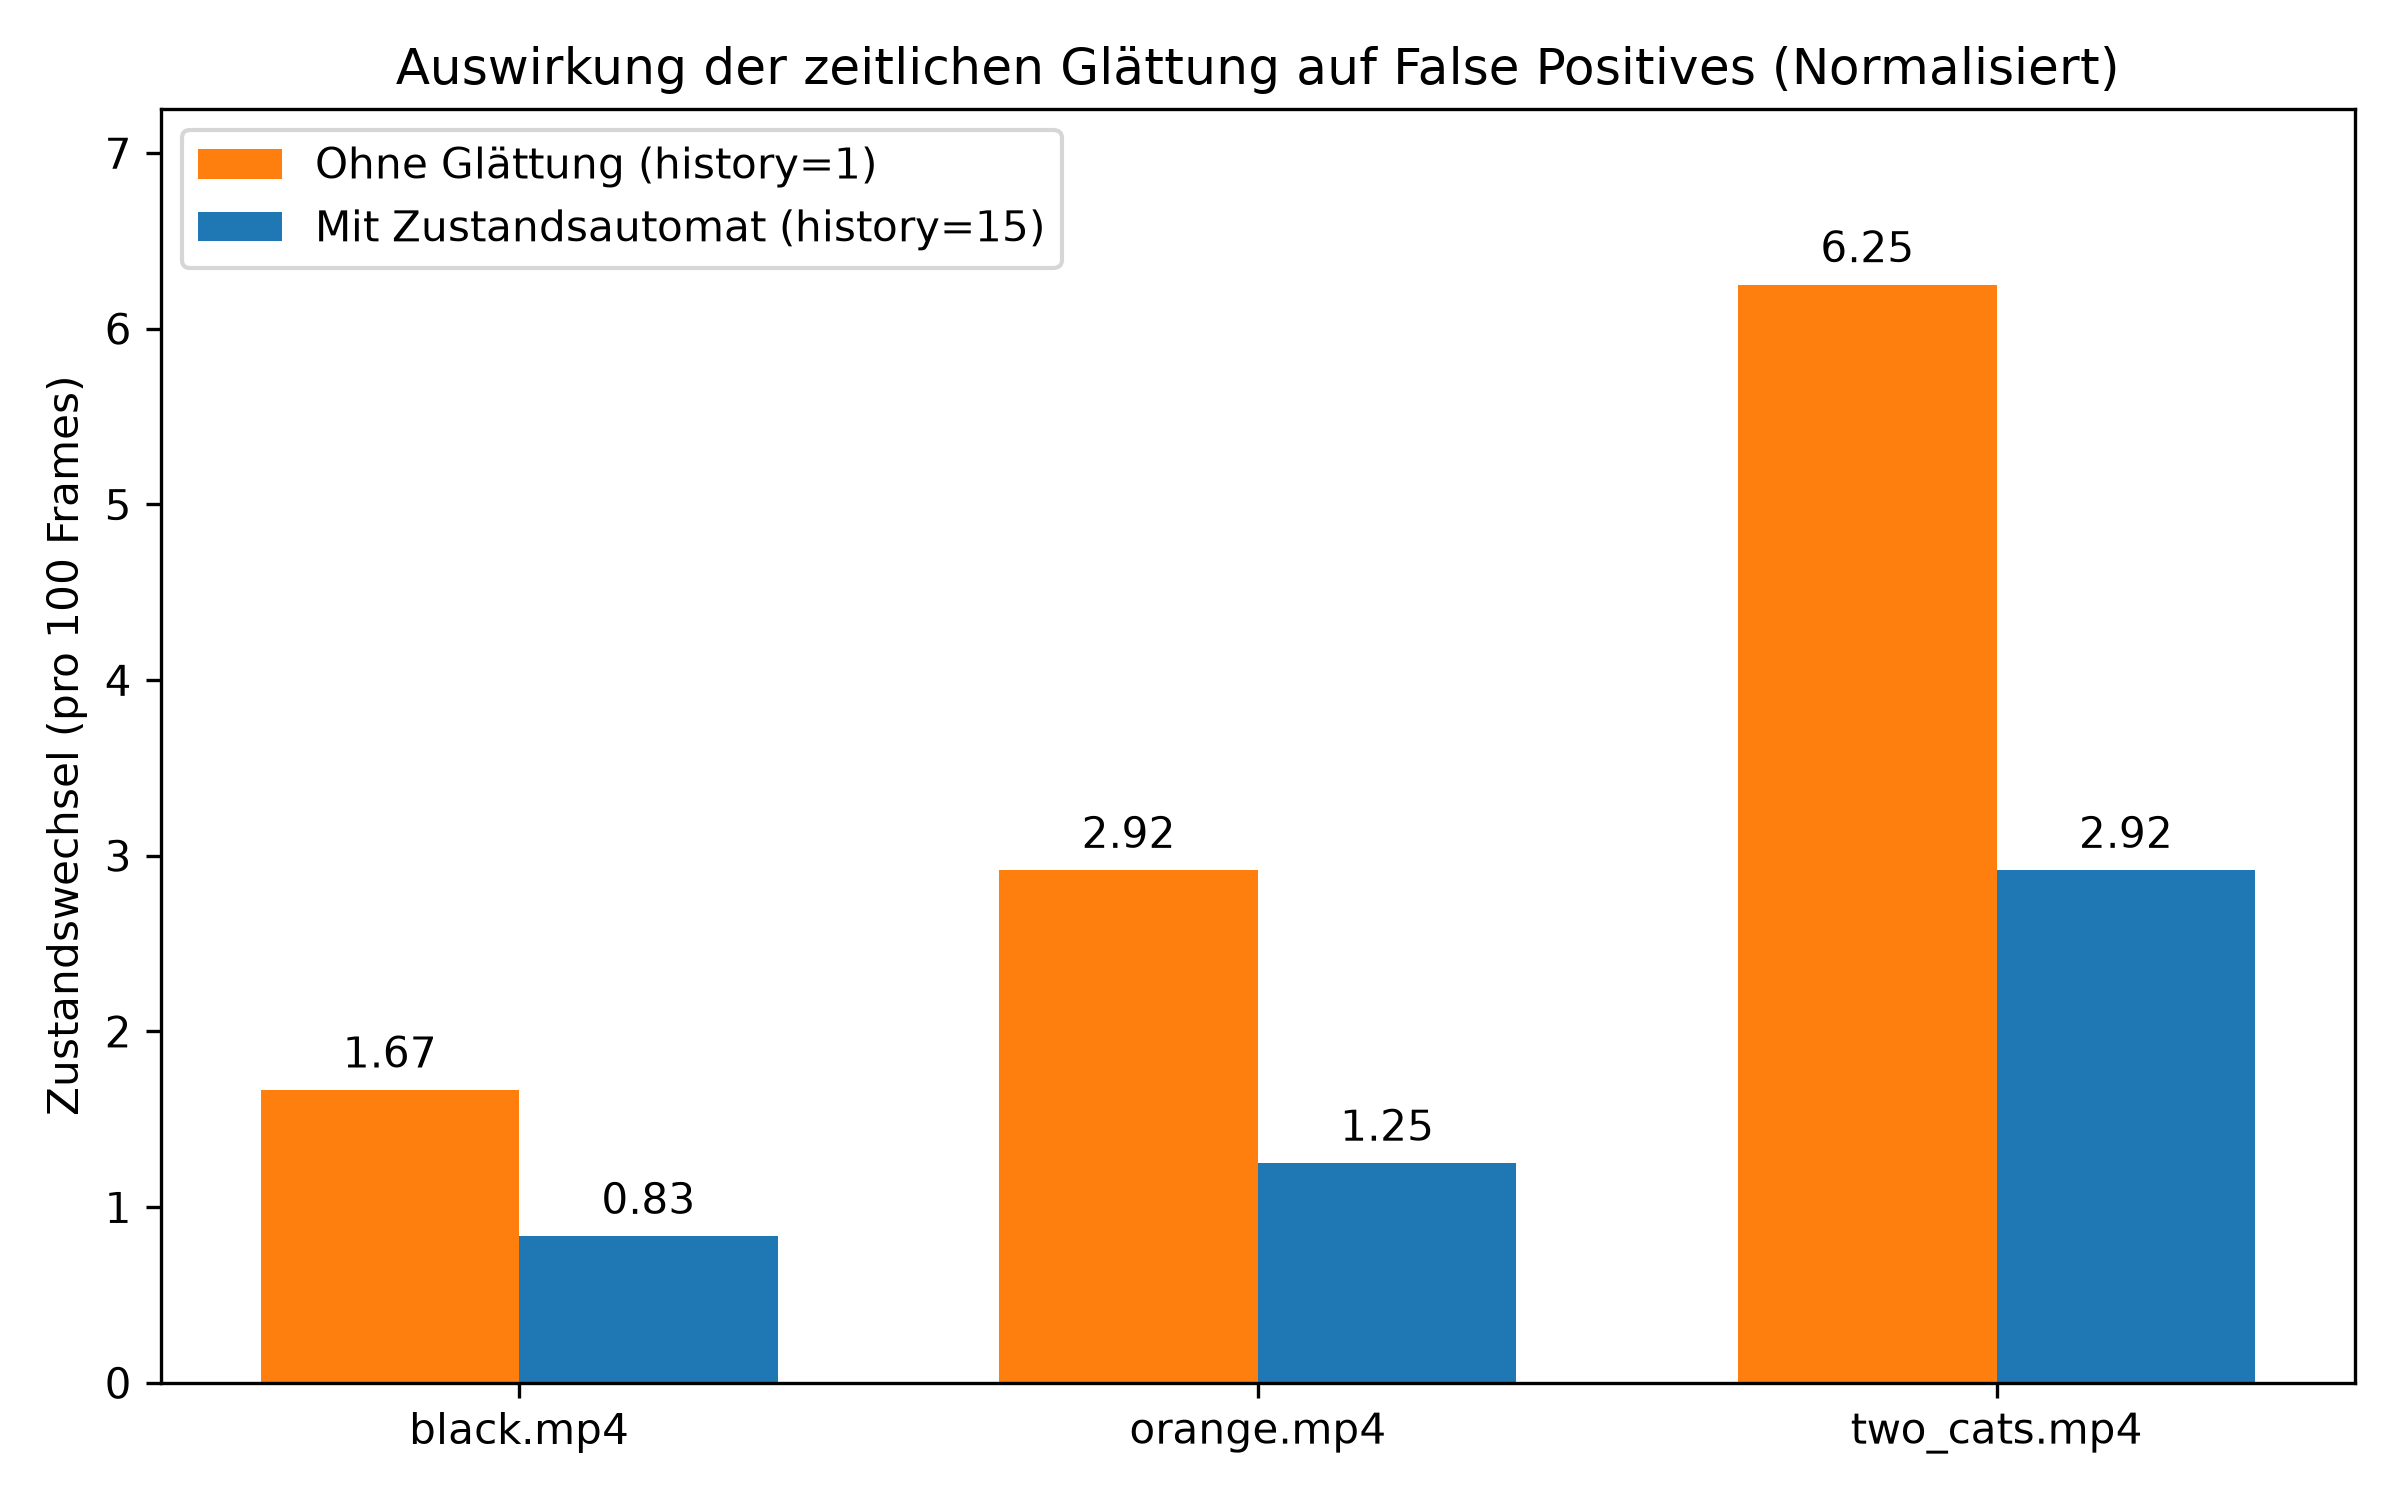
\includegraphics[width=0.9\textwidth]{images/ablation_state_changes.png}
	\caption{Zustandswechsel bei Videos ohne Beute.}
	\label{fig:ablation_states}
\end{figure}

\begin{figure}[H]
    \centering
    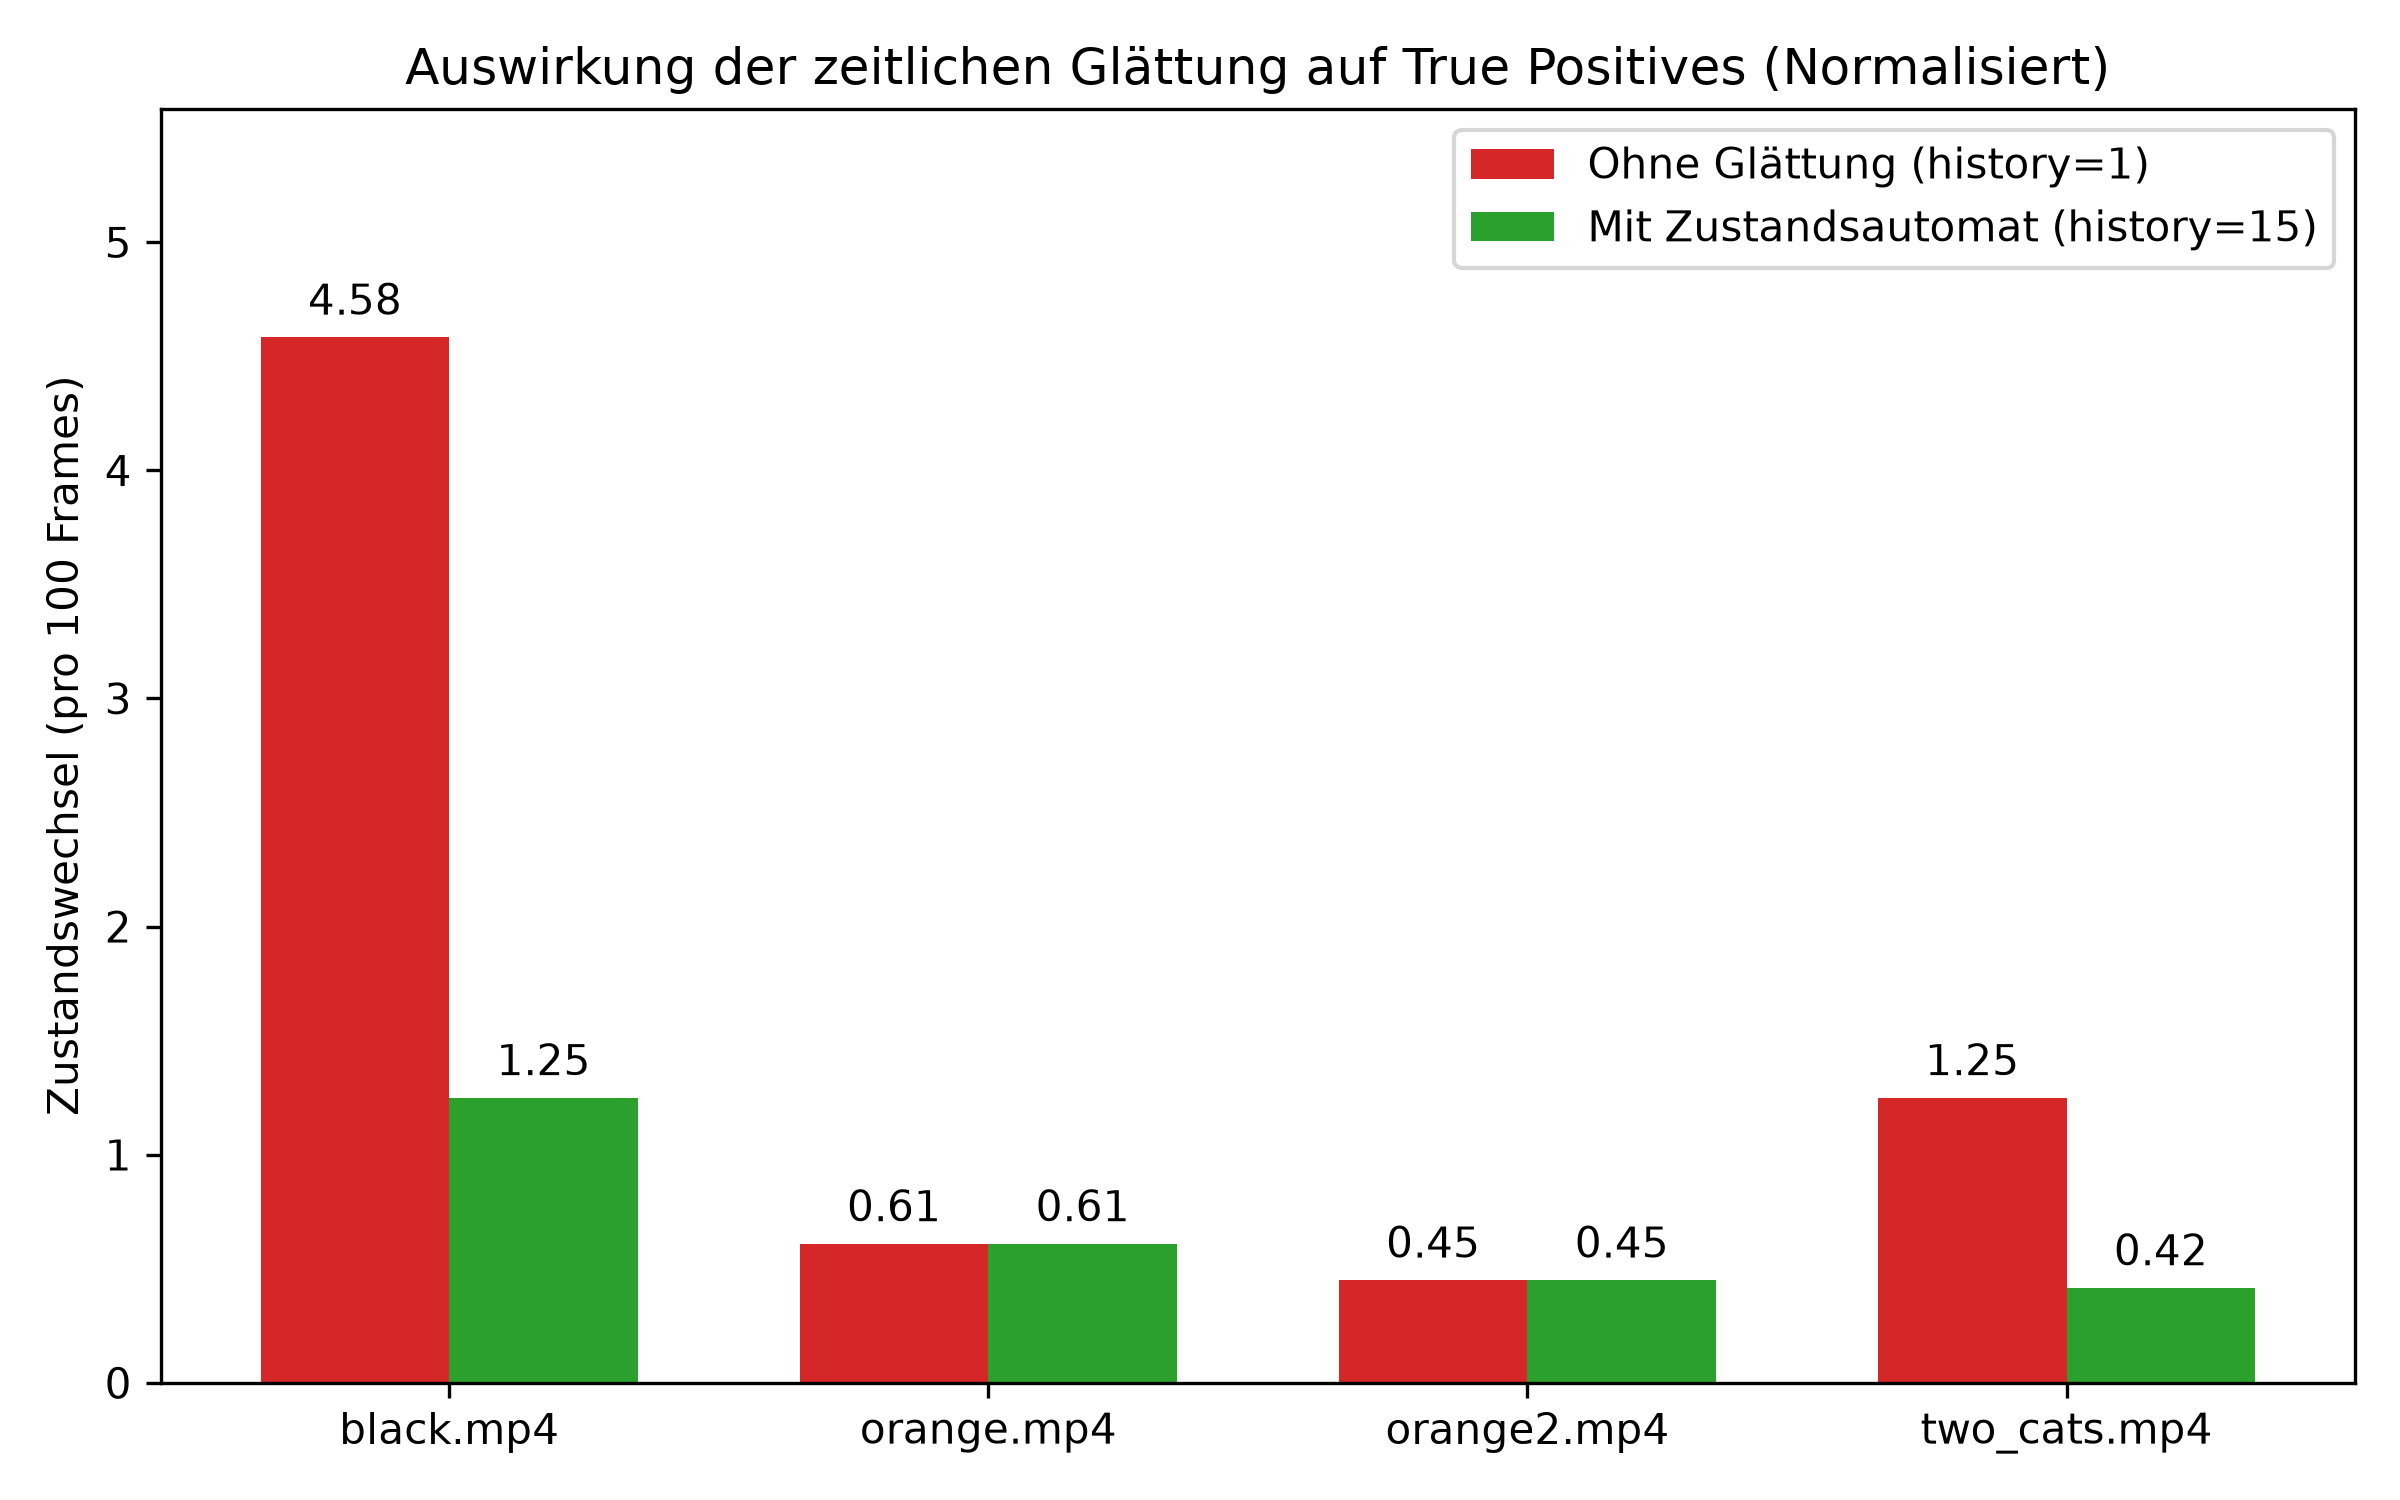
\includegraphics[width=0.9\textwidth]{images/ablation_state_changes_with_prey.png}
    \caption{Zustandswechsel bei Videos mit Beute.}
    \label{fig:ablation_states_prey}
\end{figure}

\subsection{Ablationsstudie: Relevanz des Zuschneidens}
Um isoliert beurteilen zu können wie wichtig diese Funktionalität für unser System wirklich ist, wird der Zustandsautomat völlig deaktiviert (\texttt{history\_length=1}). 

Hier wird ganz schnell klar, das System fängt an zu raten. Dadurch das nicht die vollständige Beute im Bild ist, kann das Modell keine Entscheidung treffen, egal ob mit oder ohne Beute, die Vorhersagen sind unsicher und ungenau.

\begin{figure}[H]
    \centering
    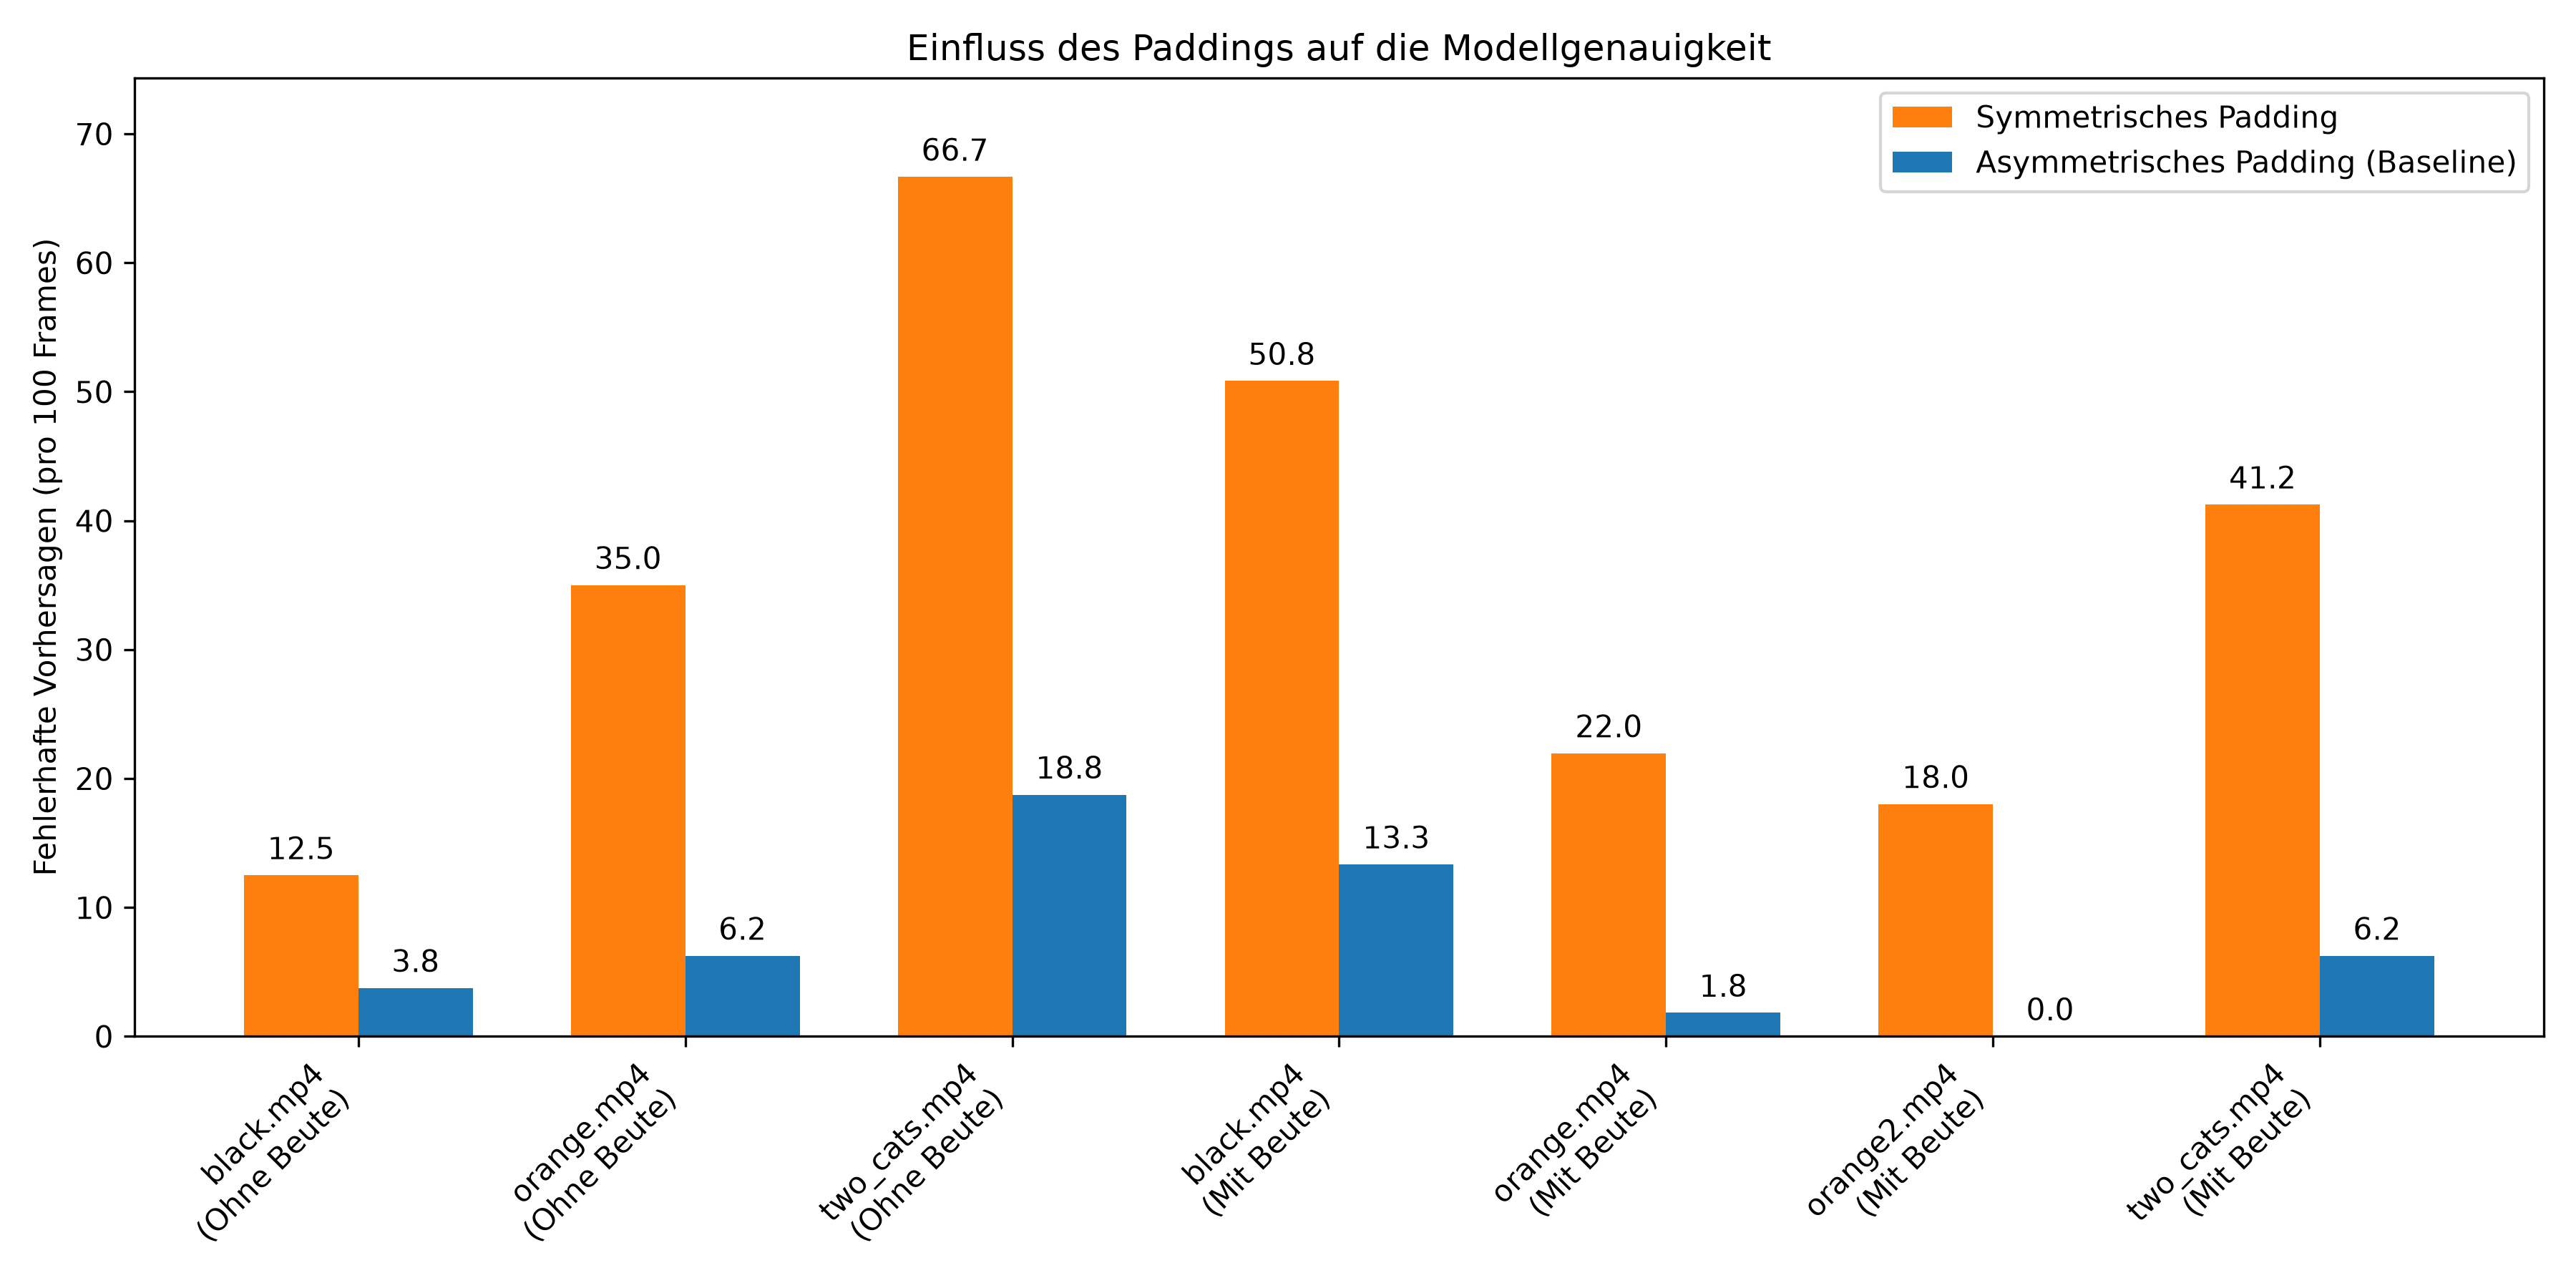
\includegraphics[width=0.7\textwidth]{images/ablation_crop_state_changes.png}
    \caption{Isolierte Auswirkung des asymmetrischen Croppings auf die rohe Systemstabilität (ohne Zustandsautomat).}
    \label{fig:ablation_crop}
\end{figure}

\subsection{Ablationsstudie: Kontrastverstärkung (CLAHE) im Klassifikator}
Da Infrarotkameras in der Nacht häufig kontrastarme Bilder liefern, wurde ein CLAHE-Filter (Contrast Limited Adaptive Histogram Equalization) in die Verarbeitungspipeline des Klassifikators integriert. Der Objektdetektor nutzt diesen Filter nicht, da er auf den originalen Graustufenbildern bereits ausreichend gut generalisiert. Um den Nutzen des Filters für die Klassifikation zu verifizieren, wurde eine dritte Ablationsstudie durchgeführt.

\begin{figure}[H]
    \centering
    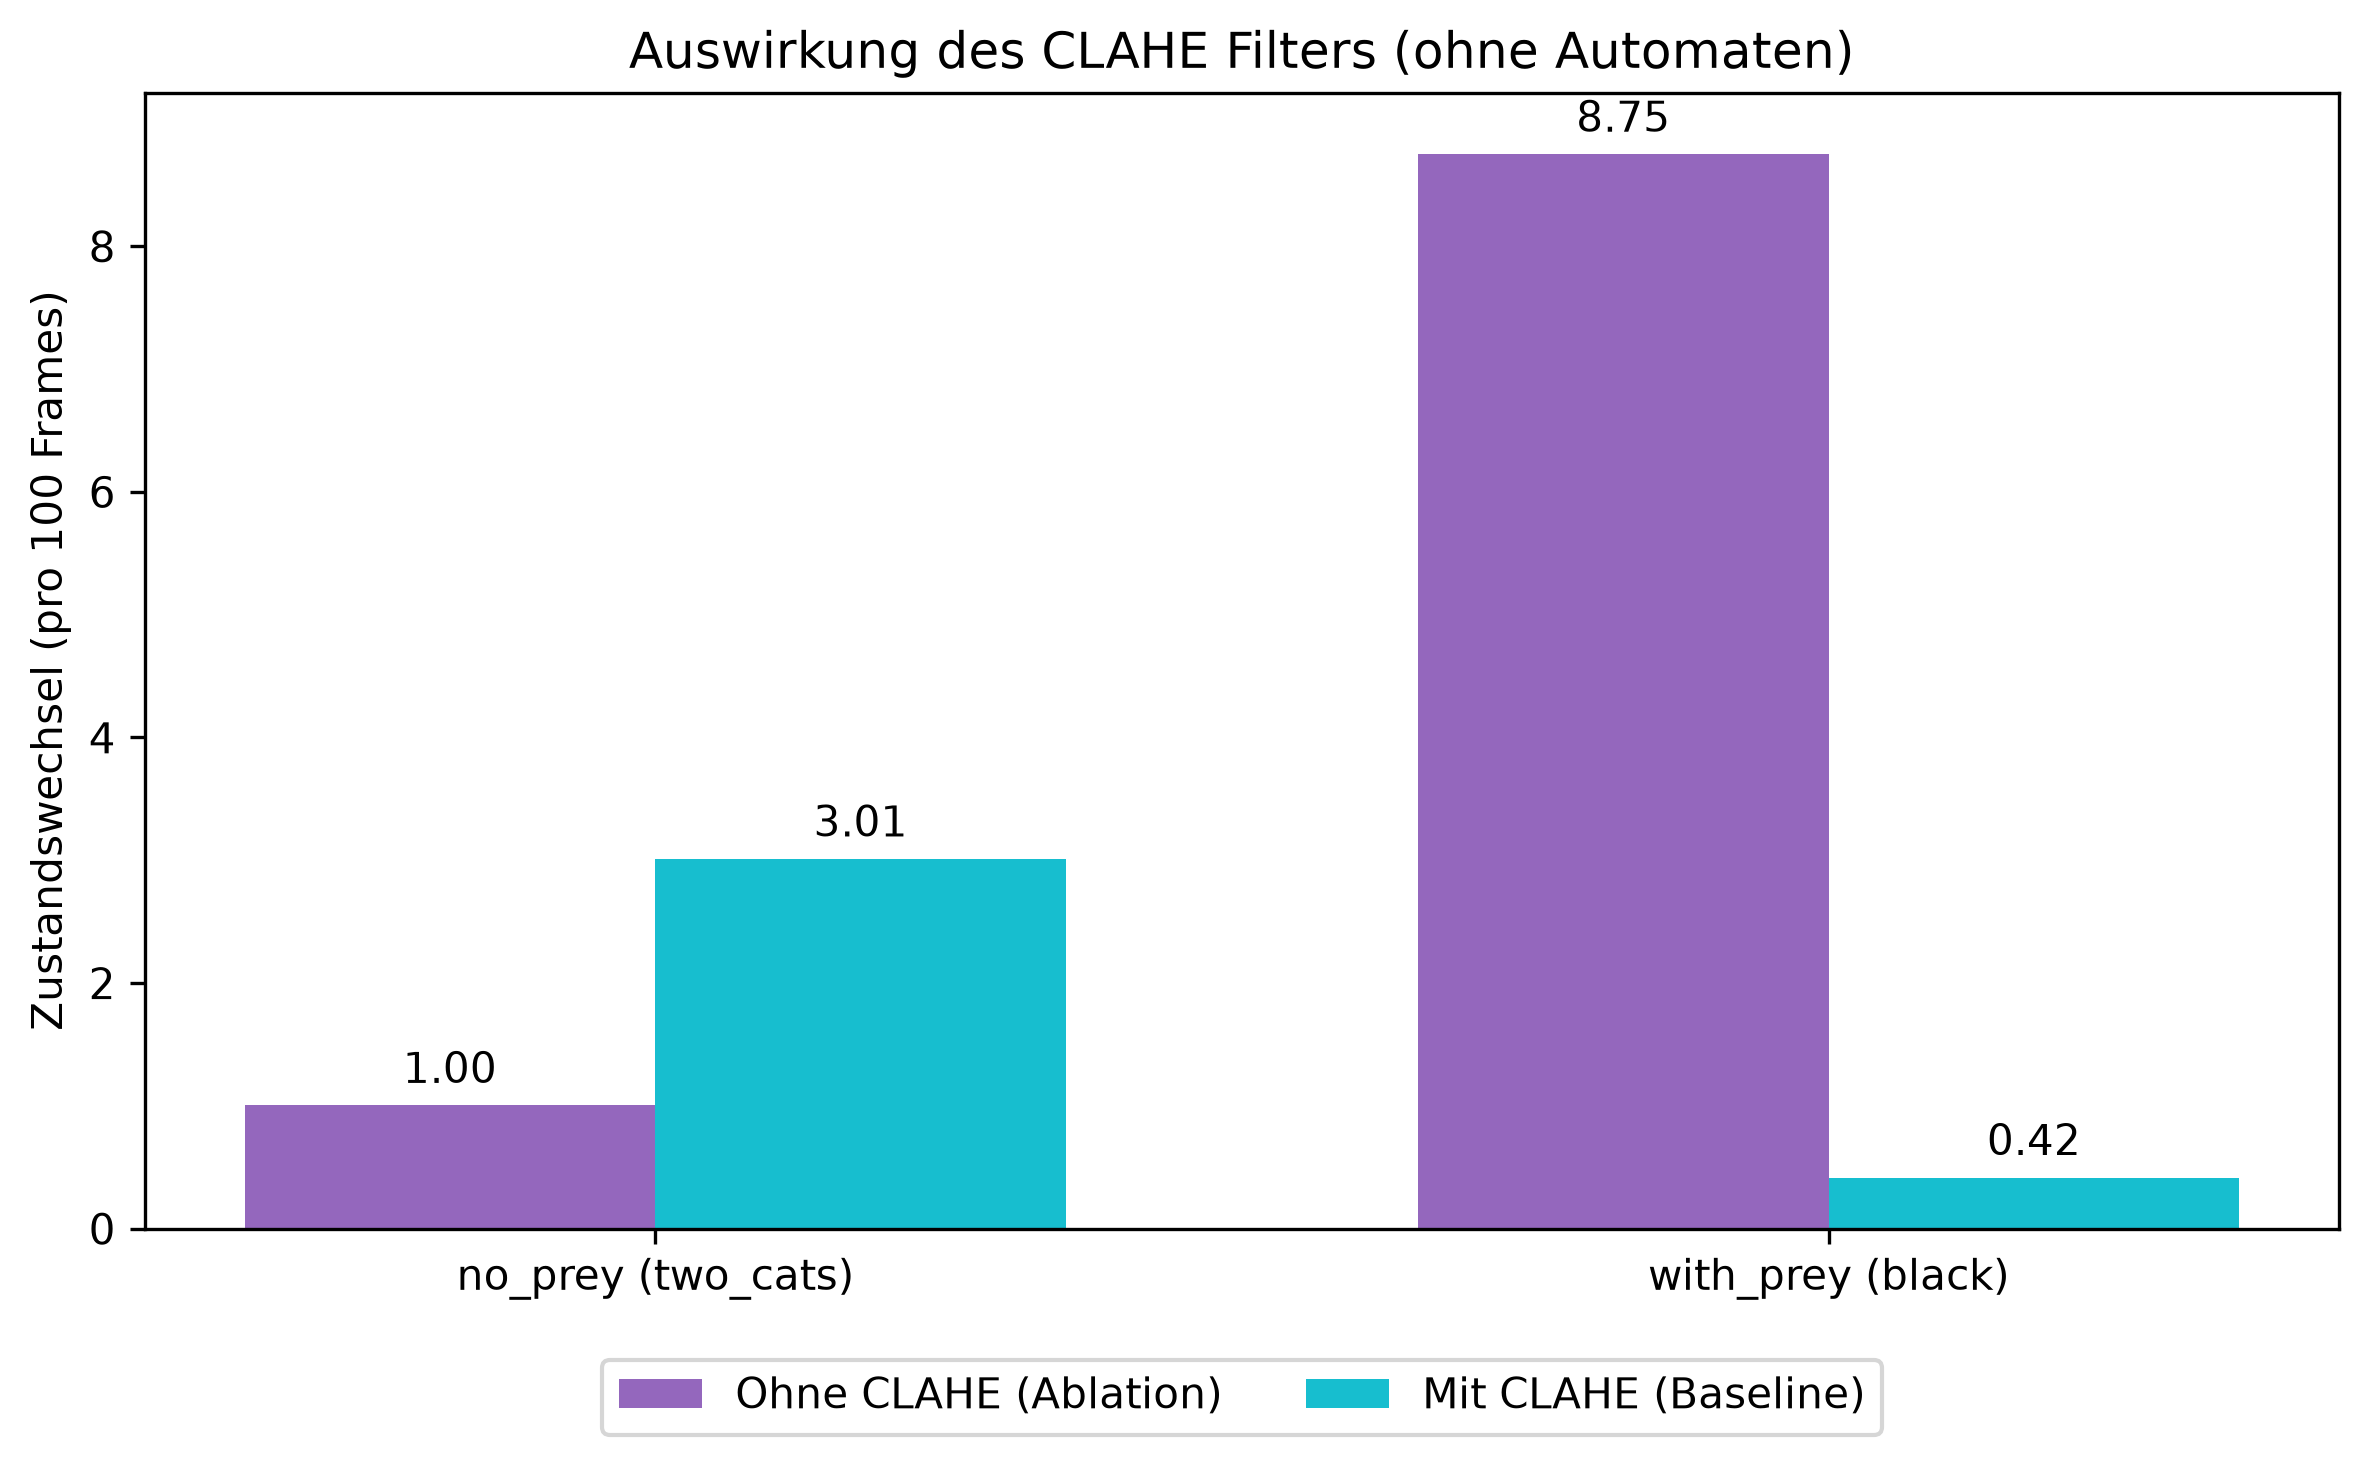
\includegraphics[width=0.9\textwidth]{images/ablation_clahe_state_changes.png}
    \caption{Vergleich der normalisierten Zustandswechsel bei Videos \emph{mit Beute} mit und ohne CLAHE-Filter im Klassifikator.}
    \label{fig:ablation_clahe}
\end{figure}

Die Ergebnisse (siehe Abbildung \ref{fig:ablation_clahe}) zeigen, dass der Filter bei Katzen ohne Beute kaum einen Unterschied macht (die Fehlalarmquote bleibt nahezu identisch). Einen massiven Einfluss hat der Filter jedoch bei Videos \emph{mit Beute} unter schwierigen Lichtbedingungen.

Besonders beim Testvideo \texttt{black.mp4} (schwarze Katze in der Nacht, die eine Beute im Maul trägt) wird der Unterschied deutlich: Mit aktiviertem CLAHE-Filter (Baseline) erkennt das System die Beute sofort und verriegelt die Klappe mit genau 1 Zustandswechsel dauerhaft. Ohne den CLAHE-Filter (Ablation) stieg die Rate auf über 2 Zustandswechsel pro 100 Frames an (insgesamt 5 Wechsel im kurzen Clip). Das bedeutet, dass das System die Klappe verriegelte, sie kurz darauf wieder entriegelte und wieder verriegelte (ein ständiges \glqq Flackern\grqq). Der Klassifikator verlor ohne den erhöhten Kontrast mehrfach die Konfidenz in die Erkennung der Beute, was im realen Einsatz dazu führen könnte, dass die Katze im falschen Moment doch mit der Maus das Haus betritt. Der CLAHE-Filter ist somit ein kritischer Baustein für die Stabilität des Systems bei Nachtaufnahmen.
